\chapter{随机搜索}
\label{chap:random-search}

要安排一批车辆的出发顺序，或者调一台模拟程序的几个开关和旋钮，每试一组方案，都只能得到一个代价数字。没有梯度，顺序和开关也谈不上求导；代价随方案的变化还可能高低起伏，朝眼前更好的方向走几步就停在一个局部低谷里。这时能做的，是决定下一批试哪些方案，以及怎样利用已经试过的结果。

第~\ref{chap:zeroth-order-optimization}章用函数值构造局部方向，仍然沿着一条路径向下走。本章换一种组织方式：不估计方向，而是管理候选。把这种方式统称为\term{随机搜索}（random search）：用随机提议产生候选，用评价结果决定保留什么，再由保留下来的信息安排后续的提议。

下面先固定问题，看清局部改善为什么会停。然后依次讨论四类方法，它们的差别在于保存什么、怎样更新：模拟退火只保存一个状态，靠接受规则决定要不要走；演化策略保存一个高斯分布，靠选择结果调整它的中心和形状；遗传算法保存一个种群，靠编码上的交叉和变异重组已有候选；粒子群让每个候选带着速度和记忆移动。

后三节处理所有方法共有的问题：候选不可行时怎么办，读数有噪声时最好记录还能不能信，结果应当怎样报告。全章反复用到两个小例子，一个是七个状态的双谷代价，一个是二维多峰函数，手算的步骤都在这些例子上进行。

\section{搜索问题}
\label{sec:rs-problem}

只能评价候选时，搜索到底在面对什么？先把目标、允许的候选和一次评价的回报固定下来，再看局部改善为什么会停滞。

\paragraph{目标、候选和一次评价}
全章考虑的问题写成
\begin{equation}
 \min_{\bm{x}\in\bm{C}}f(\bm{x}),
 \label{eq:rs-problem}
\end{equation}
其中$\bm{C}$是允许的候选集合，$f$是待最小化的代价，$f^\star$和$\bm{x}^\star$是最优值和最优解。$\bm{C}$可以是$\mathbb{R}^n$的一块区域，也可以是有限集合，比如所有长度为$n$的0--1串，或者$n$个元素的所有排列。

算法与问题之间只有一种接触方式：提交一个候选$\bm{x}$，收到一个数。这叫一次\term{评价}（evaluation）。收到的数不告诉我们$f$在别处的取值，也不带梯度或曲率。全章把预算记作$B$，表示允许的评价总次数；字母$T$留给后面的温度。

\paragraph{局部改善为什么会停}
看一个最小的例子。状态集合是$\{1,2,\ldots,7\}$，每个状态只与左右相邻的状态相连，代价是
\begin{equation}
 \bigl(f(1),f(2),\ldots,f(7)\bigr)=(3,\,1,\,3,\,5,\,2,\,0,\,2).
 \label{eq:rs-double-valley}
\end{equation}
全局最小在$x=6$，代价为$0$；$x=2$是另一个低谷，代价为$1$。两个低谷之间隔着代价为$5$的$x=4$。

规则“只走向更低的邻居”从$x=3$出发，下一步到$x=2$。在$x=2$，两个邻居的代价都是$3$，都比当前高，于是永远停在这里。从$1,2,3$出发都停在$x=2$，从$4,5,6,7$出发才能到达$x=6$。七个状态里有三个起点拿不到最优解，而算法在$x=2$上收不到任何“还有更好的地方”的信号。这就是图~\ref{fig:rs-two-landscapes}(a)。

连续变量也一样。考虑二维的Rastrigin函数
\begin{equation}
 f(\bm{x})=20+\sum_{i=1}^{2}\bigl(x_i^2-10\cos(2\pi x_i)\bigr).
 \label{eq:rs-rastrigin}
\end{equation}
全局最小在原点，$f^\star=0$。余弦项在每个整数点附近挖出一个小坑，在$[-5.12,5.12]^2$内共有$11^2=121$个局部极小点。

图~\ref{fig:rs-two-landscapes}(b)从四个起点运行梯度下降，每条路径都很快落进离起点最近的小坑。例如从$(-2.3,2.6)$出发，终点约为$(-1.99,2.98)$，那里的代价约为$12.9$。梯度下降在那里做的是对的事情，梯度也确实趋于零，只是这个驻点离全局最小还很远。

\begin{BookInlineFigure}
 \centering
 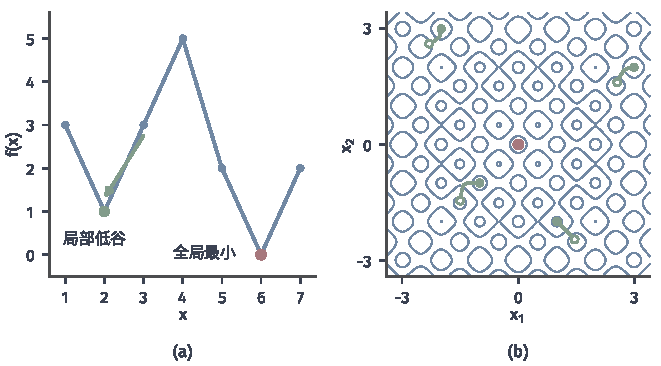
\includegraphics[width=112mm]{figures/05-optimization/05-stochastic-optimization/matplotlib/rs-two-landscapes/figure.pdf}
 \caption{两个多谷的代价。(a)七状态双谷代价~\eqref{eq:rs-double-valley}，绿色箭头是从$x=3$出发的下降，绿点是停止处，红点是全局最小。(b)二维Rastrigin函数~\eqref{eq:rs-rastrigin}的等高线（$f=8,24,40$），绿色曲线是从四个空心起点运行的梯度下降，它们都停在邻近的局部极小点（绿色实心点），红点是全局最小点。}
 \label{fig:rs-two-landscapes}
\end{BookInlineFigure}

要越过这样的障碍，算法必须做一些眼前并不划算的事：接受更差的候选，或者同时在多个地方试探。本章各方法的差别就在这里。

\paragraph{三个不同的数}
讨论算法时要分清三个数，它们经常被混为一谈。第一个是\textbf{真实目标值}$f(\bm{x})$，这是问题真正关心的量。

第二个是\textbf{读数}。评价可能含有噪声，这时收到的是
\begin{equation}
 \tilde f(\bm{x})=f(\bm{x})+\varepsilon,
 \label{eq:rs-reading}
\end{equation}
其中$\varepsilon$是这一次评价的误差。无噪声时$\tilde f=f$。第~\ref{sec:rs-noise}节之前都设无噪声。

第三个是\textbf{历史最好记录}。算法运行到第$t$次评价时，把已见的可行候选中读数最低的那个单独存下来：
\begin{equation}
 \begin{gathered}
 \bm{x}_{\mathrm{best}}^{(t)}\in\argmin\bigl\{\tilde f(\bm{x}^{(s)}):s\leq t,\ \bm{x}^{(s)}\in\bm{C}\bigr\},\\
 f_{\mathrm{best}}^{(t)}=\min_{s\leq t,\,\bm{x}^{(s)}\in\bm{C}}\tilde f(\bm{x}^{(s)}).
 \end{gathered}
 \label{eq:rs-best-record}
\end{equation}
无噪声时$f_{\mathrm{best}}^{(t)}$是真实值，而且随$t$不增。有噪声时它只是“最幸运的读数”，第~\ref{sec:rs-noise}节专门讨论这个差别。

\subsection{搜索空间}
\label{sec:rs-space}

同一个问题有不同的方式描述“从这个候选能走到哪里”。这一小节的问题是：候选的表示和移动方式怎样决定了搜索能到达什么地方？

\paragraph{三种候选，三种移动}
连续参数$\bm{x}\in\mathbb{R}^n$上最常用的移动是扰动$\bm{x}+\sigma\bm{z}$，其中$\bm{z}$是随机向量，$\sigma>0$控制尺度。一步可以到达的候选充满$\bm{x}$周围的一片区域。

二进制串$\bm{b}\in\{0,1\}^n$上的基本移动是翻位：改变一位。长度为$n$的串恰有$n$个翻位邻居，任何两个串之间相差几位，就至少需要几次翻位。

排列是把$n$个元素排成一列，$n!$种排法对应$n!$个候选。基本移动是交换两个位置上的元素。图~\ref{fig:rs-moves}把三种移动画在一起。

\begin{BookInlineFigure}
 \centering
 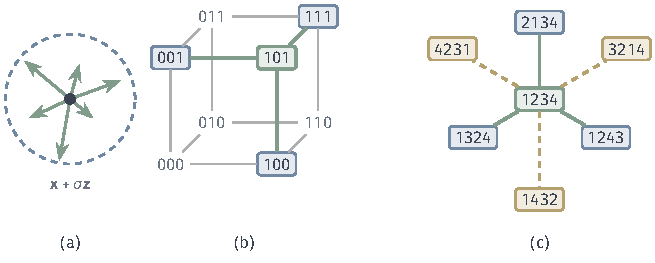
\includegraphics[width=111mm]{figures/05-optimization/05-stochastic-optimization/tikz/rs-moves/figure.pdf}
 \caption{三种候选上的移动，绿色表示当前候选及其一步移动。(a)连续参数的扰动，虚线圆表示尺度$\sigma$的量级。(b)三位二进制串构成立方体，蓝框是$101$的三个翻位邻居。(c)排列$1234$的邻居，蓝框是相邻交换，黄框和虚线是不相邻位置的交换。}
 \label{fig:rs-moves}
\end{BookInlineFigure}

把“一步能到达的候选”记为\term{邻域}（neighborhood）$\bm{N}(\bm{x})\subset\bm{C}$。邻域决定了一张图：候选是顶点，$\bm{y}\in\bm{N}(\bm{x})$就连一条边。局部低谷、爬坡路径都是相对这张图而言的，换一个邻域，低谷可能就不存在了。

\paragraph{编码要保留原问题的含义}
候选的表示必须让移动后的结果仍然有意义。例如选择问题用0--1串，第$i$位表示第$i$件物品选或不选，翻一位正是“多拿或少拿一件”，含义清楚。

把一个$0$到$15$的整数写成四位二进制，翻最高位会使整数变化$8$，翻最低位只变化$1$。从$7=0111$到相邻的$8=1000$要同时翻四位，数值上的近邻在编码上反而很远。这种表示下，翻位邻域与“数值接近”不是一回事，邻域的设计要先问清楚这一点。

\paragraph{相邻交换与任意交换}
用同一个问题比较两种邻域。平面上五个城市$A(1,4)$、$B(2,4)$、$C(3,5)$、$D(2,5)$、$E(5,0)$，距离取坐标差绝对值之和，一个访问顺序的代价是相邻两城距离之和，不返回起点。当前顺序$ABECD$的代价是
\[
 1+7+7+1=16.
\]
这条路线在中途绕向远处的$E$，然后折返，见图~\ref{fig:rs-swap-tour}(a)。

相邻交换只调换相邻的两个位置，$ABECD$的四个邻居的代价是
\[
 BAECD:17,\qquad AEBCD:18,\qquad ABCED:18,\qquad ABEDC:17.
\]
都比$16$高，所以$ABECD$是相邻交换下的局部低谷。

任意交换允许调换任何两个位置。交换$E$和$D$得到$ABDCE$，代价是
\[
 1+1+1+7=10,
\]
一步就到了五城问题的最优解，见图~\ref{fig:rs-swap-tour}(b)。

相邻交换也能到达最优解，只是要先爬坡：$ABECD\to ABCED\to ABCDE\to ABDCE$，代价依次是
\[
 16\ \to\ 18\ \to\ 12\ \to\ 10.
\]
这条路要先翻过高度为$2$的坎。同一对候选，在一种邻域下一步可达，在另一种邻域下隔着障碍。

\begin{BookInlineFigure}
 \centering
 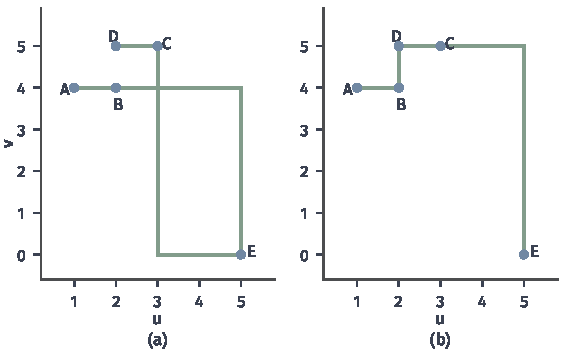
\includegraphics[width=96mm]{figures/05-optimization/05-stochastic-optimization/matplotlib/rs-swap-tour/figure.pdf}
 \caption{五城访问顺序，绿线按坐标差绝对值之和的路线画出，$u,v$是城市的横纵坐标。(a)顺序$ABECD$，长度$16$，四种相邻交换都使长度变大。(b)交换不相邻的$E$和$D$得到$ABDCE$，长度$10$。}
 \label{fig:rs-swap-tour}
\end{BookInlineFigure}

邻域并不是越大越好。五个位置时，相邻交换的邻居有$4$个，任意交换的有$10$个。任意两个排列之间，相邻交换至多需要$10$步，任意交换至多需要$4$步。

表~\ref{tab:rs-swap-neighborhood}列出这个比较。邻域大，一步能跳得远，图的直径小；代价是随机抽一个邻居时，抽到好邻居的机会被稀释，要穷举全部邻居时评价次数也更多。邻域的大小和移动尺度是算法设计中要专门决定的量，它与后面的接受规则彼此独立。

\begin{BookInlineTable}
 \centering
 \caption{$n$个元素的排列上两种交换邻域的比较，括号内是$n=5$的值。}
 \label{tab:rs-swap-neighborhood}
 \begin{tabular}{lll}
  \toprule
  & 相邻交换 & 任意交换 \\
  \midrule
  邻居个数 & $n-1$（$4$） & $n(n-1)/2$（$10$） \\
  任两排列间的最多步数 & $n(n-1)/2$（$10$） & $n-1$（$4$） \\
  是否能到达所有排列 & 能 & 能 \\
  一次移动改变的位置关系 & 小 & 可能很大 \\
  \bottomrule
 \end{tabular}
\end{BookInlineTable}

\subsection{搜索状态}
\label{sec:rs-state}

邻域回答“能走到哪里”。接下来的问题是：两次评价之间，算法手里究竟保存着什么？后面四类方法在这一点上差别最大，先把它们放在一起对比。

\paragraph{四种需要区分的对象}
\textbf{当前候选}是算法下一步移动的出发点，模拟退火就只维护这一个点。\textbf{群体成员}是同时维护的多个候选，遗传算法和粒子群属于这一类，粒子还各自带着速度。

\textbf{搜索分布参数}不是候选，而是描述“下一批候选从哪里抽”的量，例如高斯分布的中心和协方差。中心$\bm{m}$本身可能从未被评价过。\textbf{历史最好记录}是式~\eqref{eq:rs-best-record}定义的结果，它只被写入，不参与移动，除非某种算法特意使用它。

图~\ref{fig:rs-carriers}画出前三种状态，空心圆是各自的历史最好记录。表~\ref{tab:rs-state}比较它们带着什么信息。

\begin{BookInlineFigure}
 \centering
 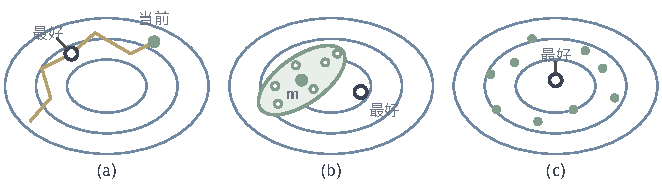
\includegraphics[width=112mm]{figures/05-optimization/05-stochastic-optimization/tikz/rs-carriers/figure.pdf}
 \caption{三种搜索状态，蓝线是目标等高线，空心圆是单独保存的历史最好记录。(a)单个当前候选（绿点）及其走过的路径（黄线），当前点可以比历史最好差。(b)搜索分布，绿点是中心$\bm{m}$，椭圆是分布的形状，空心小圆是抽到的后代，最好记录可能在椭圆外。(c)候选群体。}
 \label{fig:rs-carriers}
\end{BookInlineFigure}

\begin{BookInlineTable}
 \centering
 \caption{搜索状态承载的信息。}
 \label{tab:rs-state}
 \begin{tabular}{lll}
  \toprule
  状态 & 记住什么 & 下一批候选从哪里来 \\
  \midrule
  单个候选 & 一个点 & 这个点的邻域 \\
  搜索分布 & 中心、尺度、形状 & 从分布抽样 \\
  候选群体 & 多个点及其评价 & 成员的组合与变动 \\
  \bottomrule
 \end{tabular}
\end{BookInlineTable}

\paragraph{为什么要单独保存最好记录}
后面会看到，模拟退火有时接受更差的候选，整代替换的算法会把上一代全部丢弃。当前状态的代价因此可以上升，算法停止时手里的当前点可能比中途见过的某个点差很多。

保存记录的代价只是多存一个点。它不影响搜索的走向，却保证无噪声时交出的结果不差于任何已见的可行候选。所以无论采用什么算法，完整流程都要写上这一步。

\paragraph{与函数值方向估计的分工}
第~\ref{chap:zeroth-order-optimization}章也只用函数值：在当前点附近做差分或随机方向试探，组成梯度的估计$\hat{\bm{g}}^{(t)}$，再走一步：
\[
 \bm{x}^{(t+1)}=\bm{x}^{(t)}-\alpha^{(t)}\hat{\bm{g}}^{(t)}.
\]
它的主要对象是一个点和一个方向，分析用的是局部光滑性。

本章的主要对象是候选和选择，通常只用比较结果，也不要求$f$有导数，排列、开关这样的离散候选上根本谈不上方向。两者也有重合之处：后面第~\ref{sec:rs-es}节的高斯搜索分布，其均值的更新量可以看成平滑目标的梯度估计，这样的方法同时属于两种视角。

\section{模拟退火}
\label{sec:rs-sa}

上一节的双谷问题里，只走向更低邻居的规则停在$x=2$。这就需要回答：只维护一个状态，怎样让它有机会翻过障碍，又不至于一直乱走？\term{模拟退火}（simulated annealing，SA）的回答是：偶尔接受更差的候选，并让这种“偶尔”随时间变少。

用下山来想。一个人站在低谷里，四周都是上坡。如果他绝不上坡，就永远出不去；如果他毫不在乎坡度，就只是在地图上乱逛。合理的做法是：小坡常常愿意爬，大坡很少愿意爬，而且越到后面越不愿意爬。控制这份“愿意”的量就是温度。这个比喻到此为止：人站在山上看得到四周的坡，算法只知道它提议的那一点的代价。

\subsection{提议与接受}
\label{sec:rs-sa-accept}

一步退火由提议和接受组成。这一小节的问题是：接受规则应当怎样写，固定温度下它长期会把状态带到哪里？

\paragraph{主要思想}
一步分两半。先\textbf{提议}：从当前状态$\bm{x}$按分布$q(\bm{x},\cdot)$抽一个候选$\bm{y}$。这里设提议是对称的，即对任意$\bm{x},\bm{y}$，有$q(\bm{x},\bm{y})=q(\bm{y},\bm{x})$。

再\textbf{接受}：给定温度$T>0$，计算
\begin{equation}
 a_T(\bm{x},\bm{y})=\min\Bigl\{1,\ \exp\Bigl(-\frac{f(\bm{y})-f(\bm{x})}{T}\Bigr)\Bigr\},
 \label{eq:rs-metropolis}
\end{equation}
以概率$a_T(\bm{x},\bm{y})$移动到$\bm{y}$，否则留在$\bm{x}$。

下降或持平的提议一定被接受，上升的提议按上升量指数衰减的概率被接受。图~\ref{fig:rs-sa-acceptance}(a)画出这个函数：$T$大时曲线平缓，上坡也常被接受；$T\to0$时规则退回到只接受不上升的移动。

在双谷代价~\eqref{eq:rs-double-valley}上取$T=2$，算一次下降和一次上升。从$x=3$提议$y=2$，代价差是$-2$，接受概率为$1$。反过来，从$x=2$提议$y=3$，代价差是$+2$，接受概率为
\[
 \exp(-2/2)=\mathrm{e}^{-1}\approx0.368.
\]

上坡的代价差要除以温度才有意义。把$f$整体乘以$10$，同时把$T$乘以$10$，接受概率完全不变。所以温度的单位就是代价的单位，选温度必须看代价的尺度。

\paragraph{固定温度下的长期分布}
温度固定时，状态序列是一个马尔可夫链：下一个状态的分布只取决于当前状态。对$\bm{y}\neq\bm{x}$，一步转移的概率是
\begin{equation}
 P_T(\bm{x},\bm{y})=q(\bm{x},\bm{y})\,a_T(\bm{x},\bm{y}),
 \label{eq:rs-sa-transition}
\end{equation}
被拒绝的概率加到$P_T(\bm{x},\bm{x})$上。这个规则与下面的\term{Gibbs分布}（Gibbs distribution）紧密相关。在有限状态集合$\bm{C}$上定义
\begin{equation}
 \pi_T(\bm{x})=\frac{\exp(-f(\bm{x})/T)}{Z_T},\qquad
 Z_T=\sum_{\bm{u}\in\bm{C}}\exp(-f(\bm{u})/T).
 \label{eq:rs-gibbs}
\end{equation}
代价越低，权重越大。

\begin{theorem}[细致平衡]
\label{thm:rs-detailed-balance}
设$\bm{C}$有限，$q$对称，$T>0$。则对任意$\bm{x},\bm{y}\in\bm{C}$，
\begin{equation}
 \pi_T(\bm{x})P_T(\bm{x},\bm{y})=\pi_T(\bm{y})P_T(\bm{y},\bm{x}),
 \label{eq:rs-detailed-balance}
\end{equation}
因此$\pi_T$是转移矩阵$\bm{P}_T$的平稳分布。
\end{theorem}

\begin{proof}
$\bm{x}=\bm{y}$时两边相同。设$\bm{x}\neq\bm{y}$，不妨设$f(\bm{y})\geq f(\bm{x})$，否则交换两者的名字。这时从$\bm{y}$到$\bm{x}$是下降，$a_T(\bm{y},\bm{x})=1$，于是右边是
\[
 \pi_T(\bm{y})P_T(\bm{y},\bm{x})=\frac{\exp(-f(\bm{y})/T)}{Z_T}\,q(\bm{y},\bm{x}).
\]

从$\bm{x}$到$\bm{y}$是上升，代入式~\eqref{eq:rs-metropolis}，左边是
\[
 \begin{aligned}
 \pi_T(\bm{x})P_T(\bm{x},\bm{y})
 &=\frac{\exp(-f(\bm{x})/T)}{Z_T}\,q(\bm{x},\bm{y})\exp\Bigl(-\frac{f(\bm{y})-f(\bm{x})}{T}\Bigr)\\
 &=\frac{\exp(-f(\bm{y})/T)}{Z_T}\,q(\bm{x},\bm{y}).
 \end{aligned}
\]
由$q$的对称性，两边相等。

对式~\eqref{eq:rs-detailed-balance}关于$\bm{x}$求和，转移概率对第二个变量求和为$1$，于是
\[
 \sum_{\bm{x}}\pi_T(\bm{x})P_T(\bm{x},\bm{y})=\pi_T(\bm{y}),
\]
这正是平稳性。
\end{proof}

平稳分布存在不等于状态序列一定趋向它。若提议图连通，并且链不被周期卡住（例如某些状态有正的停留概率），状态的分布才从任何起点收敛到$\pi_T$。这一收敛结论的证明用到有限马尔可夫链的基本定理，可参考\BookChapterRef{chap:discrete-time-stochastic-processes}{卷九第3章“离散时间随机过程”}。

图~\ref{fig:rs-sa-acceptance}(b)是双谷问题的$\pi_T$。$T=2$时六号状态的概率约为$0.348$，二号状态约为$0.211$，高处的状态也有不小的份额。$T=0.5$时六号状态约为$0.850$，二号状态约为$0.115$。

\begin{BookInlineFigure}
 \centering
 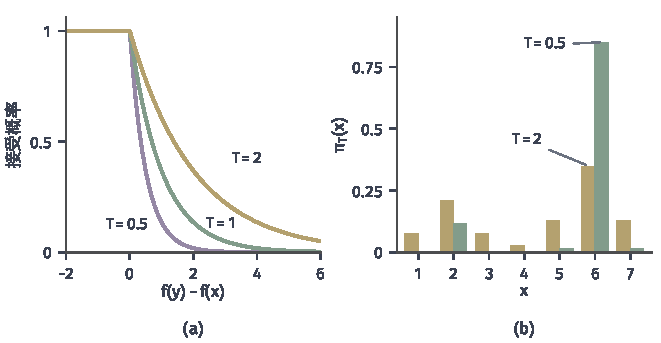
\includegraphics[width=112mm]{figures/05-optimization/05-stochastic-optimization/matplotlib/rs-sa-acceptance/figure.pdf}
 \caption{接受规则与长期分布。(a)接受概率~\eqref{eq:rs-metropolis}作为代价差的函数。(b)双谷代价~\eqref{eq:rs-double-valley}的Gibbs分布，黄色柱为$T=2$，绿色柱为$T=0.5$，温度越低，概率越集中在代价低的状态。}
 \label{fig:rs-sa-acceptance}
\end{BookInlineFigure}

温度趋于零时，$\pi_T$集中到全局最小点上。设$\bm{S}^\star$是全局最小点的集合，对任一非全局最小点$\bm{x}$和$\bm{x}^\star\in\bm{S}^\star$，比值
\[
 \frac{\pi_T(\bm{x})}{\pi_T(\bm{x}^\star)}=\exp\Bigl(-\frac{f(\bm{x})-f^\star}{T}\Bigr)\to0\qquad(T\to0^+).
\]
状态有限，所以$\pi_T(\bm{S}^\star)\to1$。这就是降温的动机：低温时的长期分布几乎全在最优解上。

问题在于“长期”。温度越低，翻越障碍越慢，走到长期分布所需的时间越长。第~\ref{sec:rs-sa-barrier}节把这件事说清楚。

\paragraph{提议不对称会怎样}
证明的最后一步用了$q$的对称性。提议不对称时，平衡关系就不再成立。看两个状态、代价相同的情形，$\pi_T=(1/2,1/2)$。

设从状态$1$总是提议$2$，而从状态$2$以$1/2$的概率提议$1$，以$1/2$的概率提议自身。代价相同，接受概率都是$1$。两状态的平稳条件是$\pi(1)\cdot1=\pi(2)\cdot\tfrac12$，于是
\[
 \pi=\Bigl(\frac13,\frac23\Bigr)\neq\Bigl(\frac12,\frac12\Bigr).
\]

要恢复目标分布，需要把提议比例放进接受概率：
\begin{equation}
 a_T(\bm{x},\bm{y})=\min\Bigl\{1,\ \exp\Bigl(-\frac{f(\bm{y})-f(\bm{x})}{T}\Bigr)\frac{q(\bm{y},\bm{x})}{q(\bm{x},\bm{y})}\Bigr\}.
 \label{eq:rs-hastings}
\end{equation}
上面的例子里，$a(1,2)=1/2$，$a(2,1)=1$，两个方向的流量都是$\pi(\cdot)\cdot\tfrac12$，$(1/2,1/2)$重新平稳。这个修正的一般讨论可参考\BookChapterRef{chap:random-sampling-integration}{卷七第14章“随机采样与积分计算”}。

\needspace{6\baselineskip}
\paragraph{变量}
下面在双谷代价上手算几步。要维护的量是：
\begin{itemize}
 \item $x^{(t)}$：当前状态，$f(x^{(t)})$是它的代价；
 \item $T^{(t)}>0$：第$t$步的温度；
 \item $x_{\mathrm{best}}$，$f_{\mathrm{best}}$：历史最好记录。
\end{itemize}

\paragraph{初始化}
选起点和初始温度，把起点记为最好记录。例中从局部低谷出发，温度每步乘以$0.9$：
\[
 x^{(0)}=2,\qquad T^{(0)}=2,\qquad T^{(t)}=2\times0.9^{t},\qquad f_{\mathrm{best}}=1.
\]
提议是等概率选左或右，超出范围时提议留在原地。

\paragraph{每轮更新}
第$t$轮依次执行以下步骤，直到用完预算。下面每一轮的提议方向和均匀随机数$u$都是事先列好的，以便逐步核对。

\begin{enumerate}
 \item 从$q(x^{(t)},\cdot)$抽候选$y$，评价$f(y)$。例中第$0$轮提议$y=1$，$f(y)=3$。
 \item 由式~\eqref{eq:rs-metropolis}计算接受概率。例中第$0$轮代价差是$2$，$T^{(0)}=2$，接受概率为$0.368$。
 \item 抽$u\sim\mathrm{U}(0,1)$，若$u<a$，令$x^{(t+1)}=y$，否则$x^{(t+1)}=x^{(t)}$。例中第$0$轮$u=0.71$，拒绝，状态仍为$2$。
 \item 若$y$可行且$f(y)<f_{\mathrm{best}}$，更新最好记录。例中第$0$轮不更新。
\end{enumerate}

表~\ref{tab:rs-sa-hand}列出前六轮。第$1$、$2$轮两次上坡都被接受，状态爬到垒顶$x=4$，代价是$5$，比记录差很多；接着第$3$、$4$轮是下坡，必然接受，第$4$轮到达$x=6$，最好记录更新为$0$。第$5$轮提议上坡到$x=7$，被拒绝。

\begin{BookInlineTable}
 \centering
 \caption{双谷代价上的前六轮，$a$是接受概率，$u$是列好的随机数。}
 \label{tab:rs-sa-hand}
 \begin{tabular}{rrrrrrrr}
  \toprule
  $t$ & $T^{(t)}$ & $x^{(t)}$ & $y$ & $f(y)-f(x^{(t)})$ & $a$ & $u$ & $f_{\mathrm{best}}$ \\
  \midrule
  $0$ & $2.000$ & $2$ & $1$ & $+2$ & $0.368$ & $0.71$ & $1$ \\
  $1$ & $1.800$ & $2$ & $3$ & $+2$ & $0.329$ & $0.25$ & $1$ \\
  $2$ & $1.620$ & $3$ & $4$ & $+2$ & $0.291$ & $0.18$ & $1$ \\
  $3$ & $1.458$ & $4$ & $5$ & $-3$ & $1$ & --- & $1$ \\
  $4$ & $1.312$ & $5$ & $6$ & $-2$ & $1$ & --- & $0$ \\
  $5$ & $1.181$ & $6$ & $7$ & $+2$ & $0.184$ & $0.62$ & $0$ \\
  \bottomrule
 \end{tabular}
\end{BookInlineTable}

最终得到$x_{\mathrm{best}}=6$，$f_{\mathrm{best}}=0$。这是特意挑选的一条幸运路径，连续爬坡两次的概率并不大，真实的成功机会要由下面的整体计算回答。

这个例子也说明了两条轨迹的区别：当前状态在第$2$轮爬到了代价$5$，比出发时差得多，而记录始终不变差。

\subsection{温度与能垒}
\label{sec:rs-sa-barrier}

温度要降到多慢，才能保证最终找到全局最小？这一小节回答这个问题，也要说明这个答案能用到什么程度。

\paragraph{能垒}
在双谷问题中，从$x=2$到代价更低的$x=6$，必须经过$x=4$。路径上的最高代价是$5$，比出发点高$4$。这个高度刻画了离开这个低谷的困难。

一般地，给定提议图和一个不是全局最小的局部低谷$\bm{x}$，考虑从$\bm{x}$到所有代价严格更低的状态的路径。路径$\bm{x}=\bm{w}_0,\bm{w}_1,\ldots,\bm{w}_k$沿提议图的边走，$f(\bm{w}_k)<f(\bm{x})$。定义\term{能垒}（energy barrier）为
\begin{equation}
 d(\bm{x})=\min_{\text{路径}}\ \max_{0\leq j\leq k}\bigl(f(\bm{w}_j)-f(\bm{x})\bigr),
 \label{eq:rs-barrier}
\end{equation}
即在所有出路中，选最省力的一条，所要爬的最大高度。全部非全局低谷的能垒中最大的一个记为$d^\star$。

双谷问题只有一个非全局低谷$x=2$。向左走不通，向右必须经过$x=4$，所以
\[
 d(2)=5-1=4,\qquad d^\star=4.
\]
图~\ref{fig:rs-barrier-depth}标出这个高度。注意能垒不等于单步的代价差：$x=2$的邻居只比它高$2$，真正要爬的是连续两步累计的$4$。

\begin{BookInlineFigure}
 \centering
 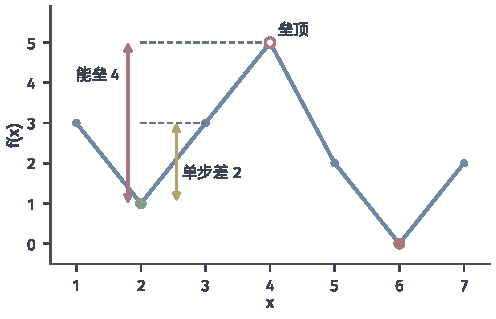
\includegraphics[width=84mm]{figures/05-optimization/05-stochastic-optimization/matplotlib/rs-barrier-depth/figure.pdf}
 \caption{双谷代价的能垒。绿点是非全局低谷$x=2$，空心红点是通往全局最小（红色实心点）必经的垒顶$x=4$。红色双箭头是能垒$d(2)=4$，黄色双箭头是一步上坡的代价差$2$。}
 \label{fig:rs-barrier-depth}
\end{BookInlineFigure}

\paragraph{对数降温的条件}
先看量级。温度为$T$时，翻过能垒$d$的那条路径大约要付出$\exp(-d/T)$的概率，所以大约要等$\exp(d/T)$步才能出去一次。$T=1$时$\mathrm{e}^4\approx55$步，$T=0.25$时已经约有$8.9\times10^{6}$步。

要让出去的机会永远不会用完，把每一步的逃逸机会加起来应当发散：
\[
 \sum_{t}\exp(-d^\star/T^{(t)})=\infty.
\]
取\term{对数降温}（logarithmic cooling）$T^{(t)}=c/\log(t+2)$，有$\exp(-d^\star/T^{(t)})=(t+2)^{-d^\star/c}$，这个级数在$c\geq d^\star$时发散，在$c<d^\star$时收敛。这就是下面定理的来历。

\begin{theorem}[对数降温下的全局收敛]
\label{thm:rs-log-cooling}
设$\bm{C}$是有限集，提议$q$对称，提议图连通，链允许原地停留。若温度取
\begin{equation}
 T^{(t)}=\frac{c}{\log(t+2)},\qquad c\geq d^\star,
 \label{eq:rs-log-cooling}
\end{equation}
则从任何起点出发，
\begin{equation}
 \lim_{t\to\infty}\mathbb{P}\bigl(\bm{x}^{(t)}\in\bm{S}^\star\bigr)=1.
 \label{eq:rs-log-cooling-limit}
\end{equation}
反之，若$0<c<d^\star$，则存在起点使这个极限不为$1$。
\end{theorem}

这一结论由Hajek于1988年给出，证明需要按代价高度逐层分析链在谷之间的转移，篇幅较长，这里不给出。下面的引理证明其中反方向的一个特殊情形，它能说明温度降得太快时发生了什么。

\begin{lemma}[降温过快时可能永远停住]
\label{lem:rs-stuck}
设$\bm{x}$的所有邻居的代价都至少比$f(\bm{x})$高$h>0$。若$T^{(t)}=c/\log(t+2)$，$0<c<h$，则从$\bm{x}$出发，状态永远不离开$\bm{x}$的概率为正。
\end{lemma}

\begin{proof}
第$t$步离开$\bm{x}$，必须接受一次上升量不小于$h$的提议，其概率不超过
\[
 \exp(-h/T^{(t)})=(t+2)^{-h/c}.
\]

记$\beta=h/c>1$。在前面各步都没有离开的条件下，第$t$步留下的概率至少是$1-(t+2)^{-\beta}$，把这些条件概率连乘，永远不离开的概率至少是
\[
 \prod_{t=0}^{\infty}\bigl(1-(t+2)^{-\beta}\bigr).
\]
由$\beta>1$，$\sum_t(t+2)^{-\beta}<\infty$，并且每个因子都大于$0$，所以这个无穷乘积大于$0$。
\end{proof}

用双谷问题具体算一次。$x=2$的两个邻居都比它高$2$，所以$h=2$。取$c=1$，提议左右各$1/2$，接受概率都是$(t+2)^{-2}$，第$t$步离开的概率恰为$(t+2)^{-2}$。于是永远留在$x=2$的概率是
\[
 \prod_{k=2}^{\infty}\Bigl(1-\frac{1}{k^2}\Bigr)=\lim_{K\to\infty}\frac{K+1}{2K}=\frac12.
\]
部分积由$(1-1/k^2)=\frac{(k-1)(k+1)}{k\cdot k}$逐项相消得到。这个算法从$x=2$出发，有一半的概率从第一步到无穷都不动。

图~\ref{fig:rs-sa-log-cooling}用转移矩阵的精确乘积算出从$x=2$出发时$x^{(t)}=6$的概率，不含抽样误差。$c=1$和$c=2$都低于$d^\star=4$，概率很快走平，到$t=2\times10^6$时分别约为$0.007$和$0.077$。$c=4$和$c=8$满足条件，概率持续上升，但到$t=2\times10^6$时也只有约$0.895$和$0.816$。

\begin{BookInlineFigure}
 \centering
 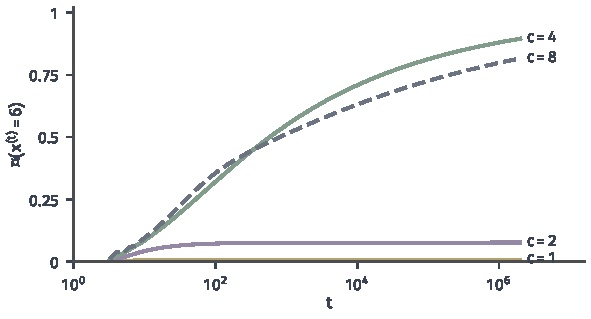
\includegraphics[width=100mm]{figures/05-optimization/05-stochastic-optimization/matplotlib/rs-sa-log-cooling/figure.pdf}
 \caption{对数降温~\eqref{eq:rs-log-cooling}下从$x=2$出发时第$t$步处于全局最小的概率，由双谷链的转移矩阵逐步相乘精确算出。$d^\star=4$，黄、紫两线的$c$小于$d^\star$，绿线取$c=4$，灰色虚线取$c=8$。横轴为对数刻度。}
 \label{fig:rs-sa-log-cooling}
\end{BookInlineFigure}

\paragraph{定理能保证什么}
这个定理的每个条件都要读准。常数$c$要覆盖能垒$d^\star$，而$d^\star$事先通常不知道。定理只对有限状态、对称连通提议成立，提议不对称或被修复过时，要重新核对。

结论是概率的极限，不是“多少步之内一定找到”。七个状态的问题，穷举只要$7$次评价，满足条件的对数降温用了两百万步仍有约一成的概率不在最优解上。$c$取得更大也不是更好：$c=8$在这个时间范围内反而不如$c=4$。

定理也不能换成任意的降温规则。按固定比例降温，$T^{(t)}=T^{(0)}\rho^t$，$0<\rho<1$，这时$\sum_t\exp(-d^\star/T^{(t)})<\infty$，定理的发散条件不满足。下一小节会看到，实际常用的正是这种规则；它能用，但不能借用上面的极限结论。

\subsection{有限预算的退火}
\label{sec:rs-sa-budget}

实际运行时，预算$B$是给定的。这一小节讨论：在$B$次评价之内，温度应当怎样安排，完整流程要包含什么？

\paragraph{三种安排}
第一种是\textbf{固定温度}，全程$T$不变，一共$B$步。第二种是\term{几何降温}（geometric cooling），每隔若干步把温度乘以比例$\rho\in(0,1)$：
\begin{equation}
 T^{[\ell]}=T^{[0]}\rho^{\ell},\qquad\ell=0,1,\ldots,K-1.
 \label{eq:rs-geometric}
\end{equation}
这里$\ell$是温度的层号，用方括号上标与迭代步区分。第三种是\textbf{分段降温}，事先列出几个温度，每个温度跑一段。

一层温度上尝试$M$次提议，共$K$层，那么一次提议就是一次评价，加上起点的一次，总评价次数是
\begin{equation}
 B=1+KM.
 \label{eq:rs-sa-budget}
\end{equation}
预算一定时，层数多则每层短，$\rho$接近$1$时降得慢。预算增加时应当把降温拉长，而不是在同样的降温后面接一段低温下的原地踏步。

\paragraph{温度的尺度}
上一小节说过，温度要和代价尺度配套。常用办法是用初始的上坡量定温度。若典型的上坡量是$\bar{\Delta}$，希望初始接受概率是$\chi_0$，那么由$\exp(-\bar{\Delta}/T^{[0]})=\chi_0$，得到
\begin{equation}
 T^{[0]}=\frac{\bar{\Delta}}{\ln(1/\chi_0)}.
 \label{eq:rs-initial-temp}
\end{equation}

双谷问题的上坡量多为$2$，取$\chi_0=0.6$，得
\[
 T^{[0]}=\frac{2}{\ln(1/0.6)}\approx3.9,
\]
可取$T^{[0]}=4$。结束温度取到上坡几乎不被接受，比如$0.1$，这时上坡量$2$的接受概率约为$2\times10^{-9}$。$\bar{\Delta}$可以先随机试若干对邻居来估计，这些试探也要记入评价次数。

提议的尺度是另一个独立的量。温度决定“接不接受”，邻域大小决定“提议走多远”。把温度调高，并不会让提议跳得更远。

\paragraph{预算内的结果}
图~\ref{fig:rs-sa-schedules}在双谷链上比较四种安排，每种安排都按预算$B$重新拉伸，并用吸收链精确计算“前$B$步内到过$x=6$”的概率。几何降温从$4$到$0.1$；分段降温依次用$4,2,1,0.5,0.25$；固定温度取$T=1$；对数降温取$c=4$。

预算为$10^4$时，几何、分段和固定温度三种安排都几乎必然到过全局最小，只有对数降温的概率约为$0.80$。对数降温在小预算时略占优势，到了大预算反而落后：它在高温停留很短，后面长时间逗留在约$0.5$的低温，翻过能垒的机会稀少。

\begin{BookInlineFigure}
 \centering
 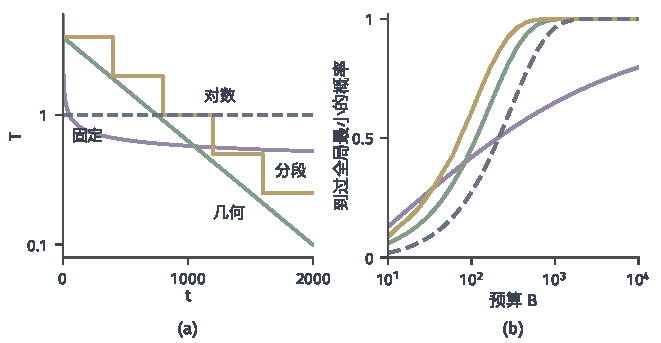
\includegraphics[width=112mm]{figures/05-optimization/05-stochastic-optimization/matplotlib/rs-sa-schedules/figure.pdf}
 \caption{双谷链上的降温安排比较。紫线为对数降温$c=4$，绿线为几何降温（$4\to0.1$），黄线为分段降温，灰色虚线为固定温度$T=1$。(a)预算$B=2000$时的温度，纵轴对数刻度。(b)预算$B$之内到过全局最小的精确概率。}
 \label{fig:rs-sa-schedules}
\end{BookInlineFigure}

这里要分清两个量。“到过”对应最好记录；“结束时停在那里”对应当前状态。预算$10^4$时，结束时处于$x=6$的概率，几何降温约为$0.79$，分段降温约为$0.75$，对数降温约为$0.71$，固定温度$T=1$约为$0.57$。固定温度下最好记录几乎一定拿到最优，当前状态却只有$\pi_1(6)\approx0.57$。

这也回答了为什么最好记录必须写进流程：不写它，固定温度下交出的当前状态有四成多的概率不是最优解。

\paragraph{完整流程}
把前面的决定合起来，一次带重启的退火这样组织。先确定预算$B$，试探代价尺度，由式~\eqref{eq:rs-initial-temp}定$T^{[0]}$，选结束温度、比例$\rho$和每层步数$M$，使总评价满足预算。

然后运行提议、接受和记录更新，每完成一层就降温。一次退火结束后，若预算还有剩余，就从新的起点重新开始，保留全局的最好记录。若单次运行成功的概率是$p$，独立重启$K$次，至少成功一次的概率是
\begin{equation}
 1-(1-p)^K.
 \label{eq:rs-restart}
\end{equation}
例如$p=0.2$，$K=5$，得到$1-0.8^5\approx0.67$。把预算切成几次短运行，单次的$p$会变小，所以切多少份要依问题试验确定。

图~\ref{fig:rs-sa-path}是二维Rastrigin函数上一次预算为$3000$的运行。高温阶段当前点在各个小坑之间跳动，代价可以高到几十；温度降低后渐渐落入一个小坑，后期几乎不再接受上坡。这次运行的最好记录为$(-0.004,0.034)$，代价约为$0.23$。

这是这一次运行得到的结果，换一个种子结果就可能不同。在有限预算下，这样的方法要按运行结果的分布评价，不能因为存在对数降温的极限定理，就说它“能收敛到全局最优”。第~\ref{sec:rs-evaluation}节回到如何评价的问题。

\begin{BookInlineFigure}
 \centering
 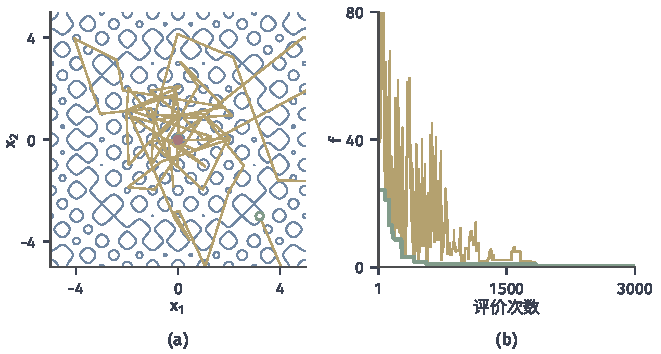
\includegraphics[width=112mm]{figures/05-optimization/05-stochastic-optimization/matplotlib/rs-sa-path/figure.pdf}
 \caption{二维Rastrigin函数~\eqref{eq:rs-rastrigin}上的一次模拟退火，高斯提议$\sigma=0.8$，温度从$25$几何下降到$0.05$，$B=3000$，种子固定。(a)蓝线是等高线，黄线是当前状态的路径（每隔$18$步取一点），空心圆是起点，绿点是最好记录，红点是全局最小点。(b)黄线是当前状态的代价，绿线是最好记录的代价。}
 \label{fig:rs-sa-path}
\end{BookInlineFigure}

\section{演化策略}
\label{sec:rs-es}

模拟退火只有一个状态，提议的形状事先给定。连续变量上还有一种选择：不维护候选，而维护一个“下一批候选从哪里抽”的分布，并让评价结果来修改这个分布。怎样根据一批候选的好坏，调整分布的中心、尺度和形状？这类方法称为\term{演化策略}（evolution strategy，ES）。

一代的流程是：抽出若干候选（称为\term{后代}，offspring），评价，选出较好的（称为\term{亲代}，parents），再由亲代决定下一代的分布。这里的“亲代”“后代”只是名称，所有内容都由下面的公式定义。本节用$\mu$表示亲代个数，$\lambda$表示后代个数，两者都是正整数，不再表示强凸常数和乘子。

\subsection{变异与重组}
\label{sec:rs-es-mutation}

后代从亲代而来。这一小节的问题是：单个后代怎样产生，有多个亲代时又怎样利用它们？

\paragraph{高斯变异}
从亲代$\bm{x}$产生后代的基本方式是加一个高斯扰动：
\begin{equation}
 \bm{y}=\bm{x}+\sigma\bm{z},\qquad\bm{z}\sim\mathcal{N}(\bm{0},\bm{I}),
 \label{eq:rs-mutation}
\end{equation}
称为\term{高斯变异}（Gaussian mutation）。步长$\sigma>0$控制扰动的整体尺度，各向同性指的是所有方向的扰动幅度相同。

用全卷的二次例子$f(\bm{x})=\tfrac12(x_1^2+9x_2^2)$手算一次。在$\bm{x}=(9,1)$处，$f=45$。取$\sigma=1$，抽到$\bm{z}=(-0.8,-0.5)$，后代是$(8.2,0.5)$，代价为
\[
 \tfrac12(67.24+2.25)\approx34.75,
\]
比亲代好，留下。抽到$\bm{z}=(-0.2,0.9)$时，后代是$(8.8,1.9)$，代价约为$54.97$，变差，丢弃。这样只保留变好的结果，就是最简单的$(1+1)$策略，名字的含义下一小节解释。

\paragraph{各向同性的局限}
这个目标在$x_2$方向比$x_1$方向陡$9$倍。图~\ref{fig:rs-es-isotropic}(a)在$(9,1)$周围取$\sigma=2$抽$60$个后代，绿点代价下降，红圈代价上升。圆形的云团和拉长的等高线不匹配：往$x_2$方向稍远一点就越出了等高线。

图~\ref{fig:rs-es-isotropic}(b)用$8\times10^5$个样本估计改善的概率。$\sigma$趋于零时，等高线局部接近直线，改善概率趋于$1/2$；$\sigma$增大，各向同性的抽样在$\sigma\approx2$时约为$0.31$，而沿等高线拉伸的抽样（两个方向的标准差比为$3:1$，面积相同）仍约有$0.42$。

\begin{BookInlineFigure}
 \centering
 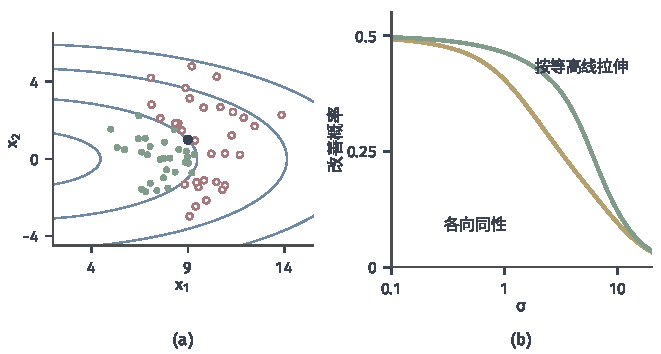
\includegraphics[width=112mm]{figures/05-optimization/05-stochastic-optimization/matplotlib/rs-es-isotropic/figure.pdf}
 \caption{$f=\tfrac12(x_1^2+9x_2^2)$上的变异，亲代在$(9,1)$。(a)蓝线是等高线，深色点是亲代，$\sigma=2$的各向同性后代中绿点改善、红圈变差。(b)改善概率随$\sigma$的变化，黄线为各向同性抽样，绿线的两个坐标标准差分别为$\sqrt3\sigma$和$\sigma/\sqrt3$，由固定种子抽样估计。}
 \label{fig:rs-es-isotropic}
\end{BookInlineFigure}

所以固定的圆形变异有两个问题：$\sigma$要随进展变化，形状也应当贴合地形。后面两小节分别解决。

\paragraph{多个亲代：选一个还是合成一个}
有多个亲代时，有两种产生后代的方式。一种是每次选一个亲代，在它周围变异。另一种是先把亲代合成一个点，称为\term{重组}（recombination），再从这一点变异，比如取权重$w_1\geq\cdots\geq w_\mu>0$，$\sum_iw_i=1$，按代价从好到差排序，
\begin{equation}
 \bm{m}=\sum_{i=1}^{\mu}w_i\bm{x}_{i:\lambda},
 \label{eq:rs-recombination}
\end{equation}
下标$i:\lambda$表示$\lambda$个后代中第$i$好的那个。

取两个亲代手算。$\bm{x}_{1:\lambda}=(7,-0.8)$的代价为$27.38$，$\bm{x}_{2:\lambda}=(8,0.6)$的代价为$33.62$。权重取$(3/4,1/4)$，重组后得到
\[
 \bm{m}=\tfrac34(7,-0.8)+\tfrac14(8,0.6)=(7.25,-0.45),\qquad f(\bm{m})\approx27.19.
\]
重组点比两个亲代都好。

原因在于两个亲代沿$x_2$的偏差一正一负，平均后相互抵消，$x_2$方向的代价又贵，于是抵消的好处很大。这是重组的一种效果：把各个亲代中互不相关的扰动平均掉，保留它们共有的移动。这也不是必然的结果，两个亲代偏差同号时重组就没有这个好处。

\paragraph{两类量}
演化策略中有两类量要分开。一类是\textbf{待优化变量}，就是候选$\bm{x}$本身，提交给$f$评价。另一类是\textbf{策略参数}，如$\sigma$和后面的协方差，它们决定怎样抽样，不提交给$f$，却随代更新。

\subsection{亲代选择}
\label{sec:rs-es-selection}

一代产生了$\lambda$个后代，下一代的亲代应从谁中选？这一小节比较两种规则，并说明它们各自能保证什么。

\paragraph{两种规则}
$(\mu+\lambda)$策略从$\mu$个旧亲代和$\lambda$个后代的并集中选出最好的$\mu$个。$(\mu,\lambda)$策略只从$\lambda$个后代中选最好的$\mu$个，旧亲代全部丢弃，因此要求$\lambda\geq\mu$；$\lambda=\mu$时全部后代都入选，就没有选择了，实际要取$\lambda>\mu$。

前面的$(1+1)$就是一个亲代、一个后代，留下较好者的规则。

\begin{theorem}[保留亲代时最好值不增]
\label{thm:rs-elitist}
设评价无噪声，亲代的代价是准确的。采用$(\mu+\lambda)$选择时，记第$t$代亲代中的最小代价为$f_{\min}^{(t)}$，则
\begin{equation}
 f_{\min}^{(t+1)}\leq f_{\min}^{(t)},\qquad t=0,1,\ldots.
 \label{eq:rs-elitist}
\end{equation}
\end{theorem}

\begin{proof}
第$t$代代价最小的亲代属于第$t+1$代选择的并集。选择取并集中最好的$\mu$个，所以并集的最小代价一定入选，而并集的最小代价不超过$f_{\min}^{(t)}$。
\end{proof}

\paragraph{这个保证的边界}
最好值不增不等于在进步，更不等于走向全局最优。把$(1+1)$规则放在双谷问题上，变异只提议左右相邻的状态，从$x=2$出发，两个邻居都更差，永远不会有后代入选。式~\eqref{eq:rs-elitist}成立，算法却永远停在$f=1$。

高斯变异的支撑是全空间，任何点都有正的概率被抽到，但一次跳过很宽的障碍的概率随距离指数下降，这个正概率在有限预算下没有意义。旧亲代保留也可能拖累搜索：一个特别好的旧亲代长期占据位置，后代都比不过它，$\sigma$的调整也因此失去依据。

\paragraph{两种规则的对比}
图~\ref{fig:rs-es-plus-comma}(a)在二次目标上用固定的$\sigma=0.5$，$\lambda=5$，$\mu=1$。保留亲代时曲线单调下降，到第$80$代代价约为$0.0026$。整代替换时，每一代的亲代都是新的，到了尺度$\sigma$能分辨的精度后就在附近上下波动，第$80$代当前代价约为$0.10$，只有其最好记录（虚线）约为$0.0016$。

图~\ref{fig:rs-es-plus-comma}(b)换到二维Rastrigin函数，$\sigma=0.45$，$40$次独立运行取中位数，起点$(2,2)$，代价为$8$。保留亲代时前期被小坑拦住，改进较慢；整代替换的最好记录（虚线）早期下降更快，因为当前点可以连续穿过小坑，但它的当前代价一直在$10$到$14$之间摆动，到$200$代时中位数约为$14$，而保留亲代的中位数约为$0.39$，整代替换的最好记录约为$0.85$。

\begin{BookInlineFigure}
 \centering
 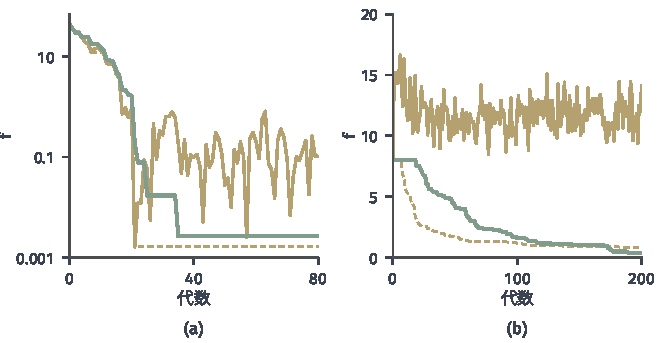
\includegraphics[width=112mm]{figures/05-optimization/05-stochastic-optimization/matplotlib/rs-es-plus-comma/figure.pdf}
 \caption{保留亲代（绿线）与整代替换（黄色实线为当前亲代的代价，黄色虚线为其历史最好）的对比，$\mu=1$，$\lambda=5$，$\sigma$固定。(a)$f=\tfrac12(x_1^2+9x_2^2)$，$\sigma=0.5$，一次运行，纵轴对数刻度。(b)二维Rastrigin函数，$\sigma=0.45$，$40$次运行的中位数，线性纵轴。}
 \label{fig:rs-es-plus-comma}
\end{BookInlineFigure}

\begin{BookInlineTable}
 \centering
 \caption{两种亲代选择的对比。}
 \label{tab:rs-plus-comma}
 \begin{tabular}{lll}
  \toprule
  & $(\mu+\lambda)$ & $(\mu,\lambda)$ \\
  \midrule
  旧亲代 & 与后代竞争 & 全部丢弃 \\
  无噪声时亲代最好值 & 不增 & 可能上升 \\
  是否需要单独保存最好记录 & 不必（已含在亲代中） & 必须 \\
  好亲代长期占位 & 可能 & 不会 \\
  \bottomrule
 \end{tabular}
\end{BookInlineTable}

两种规则都需要配合下面的尺度和形状更新。选择只决定谁留下，走多远、朝哪个形状抽，还要靠策略参数。

\subsection{协方差适应}
\label{sec:rs-es-cma}

圆形的抽样不贴合地形，这一小节的问题是：怎样让抽样分布的形状从评价结果中学出来？

\paragraph{主要思想}
把圆形的扰动换成椭圆形，后代从下式抽取：
\begin{equation}
 \bm{x}_i^{(t+1)}=\bm{m}^{(t)}+\sigma^{(t)}\bm{y}_i,\qquad\bm{y}_i\sim\mathcal{N}(\bm{0},\bm{\Sigma}^{(t)}),\quad i=1,\ldots,\lambda.
 \label{eq:rs-cma-sample}
\end{equation}
这里$\bm{m}^{(t)}$是分布的中心，$\sigma^{(t)}$是整体尺度，对称正定矩阵$\bm{\Sigma}^{(t)}$描述形状。\term{协方差矩阵适应演化策略}（covariance matrix adaptation evolution strategy，CMA-ES）的思路是：让“抽到好后代的那些位移”的分布，成为下一代的抽样分布。

好后代位移的方向多次出现，就说明沿那个方向走有好处，下次沿这个方向多抽一些。可以这样对应：等高线是一条拉长的山谷，中心$\bm{m}$是当前站立的位置，$\bm{\Sigma}$是下一次向四周探路时的步幅分配，把更多的步幅给谷底的走向。

具体的目标用旋转过的椭圆：
\begin{equation}
 f(\bm{x})=\frac12\bm{x}^\top\bm{A}\bm{x},\qquad
 \bm{A}=\begin{bmatrix}5&-4\\-4&5\end{bmatrix}.
 \label{eq:rs-rotated}
\end{equation}
$\bm{A}$的特征值是$1$和$9$，对应的特征方向是$(1,1)$和$(1,-1)$，所以山谷沿$(1,1)$方向。这种倾斜不能靠给两个坐标各设一个步长来表示，必须有非对角元。

更新分三步。第一步按评价排序，只用排序不用代价的数值，取前$\mu$个$\bm{y}_{i:\lambda}$。中心向它们的加权平均移动，权重$w_i$为正，和为$1$：
\begin{equation}
 \bm{y}_w=\sum_{i=1}^{\mu}w_i\bm{y}_{i:\lambda},\qquad
 \bm{m}^{(t+1)}=\bm{m}^{(t)}+\sigma^{(t)}\bm{y}_w.
 \label{eq:rs-cma-mean}
\end{equation}

第二步累积一条路径。一代的$\bm{y}_w$里有随机成分，但真实的好方向会在连续几代中重复出现。把连续几代的$\bm{y}_w$累加起来，得到\term{演化路径}（evolution path）：
\begin{equation}
 \bm{p}_c^{(t+1)}=(1-c_c)\bm{p}_c^{(t)}+\sqrt{c_c(2-c_c)\mu_w}\,\bm{y}_w,\qquad
 \mu_w=\frac{1}{\sum_iw_i^2},
 \label{eq:rs-cma-pc}
\end{equation}
其中$c_c\in(0,1]$决定记忆长度。$\mu_w$是有效亲代数，权重越平均越大。系数$\sqrt{c_c(2-c_c)\mu_w}$的来历在下一小节解释。

第三步更新协方差，把三部分加起来：
\begin{equation}
 \bm{\Sigma}^{(t+1)}=(1-c_1-c_\mu)\bm{\Sigma}^{(t)}
 +c_1\bm{p}_c^{(t+1)}\bigl(\bm{p}_c^{(t+1)}\bigr)^\top
 +c_\mu\sum_{i=1}^{\mu}w_i\bm{y}_{i:\lambda}\bm{y}_{i:\lambda}^\top.
 \label{eq:rs-cma-cov}
\end{equation}
第一部分是旧的形状，第二部分来自路径方向，称为秩一更新，第三部分是这一代选中位移的加权协方差，称为秩$\mu$更新。

式~\eqref{eq:rs-cma-cov}的$\bm{y}_{i:\lambda}$是相对旧中心的位移，用的是旧的$\bm{m}$。如果用新的$\bm{m}$，等于把这一代沿平均方向的进展减掉了，协方差就只记录了后代之间的散布，看不出朝哪边走有好处。

\paragraph{协方差保持正定}
抽样要求$\bm{\Sigma}$正定，下面的引理说明正权重时自动满足。

\begin{lemma}[协方差更新保持正定]
\label{lem:rs-cma-pd}
设$\bm{\Sigma}^{(t)}$对称正定，$c_1,c_\mu\geq0$，$c_1+c_\mu<1$，$w_i>0$。则由式~\eqref{eq:rs-cma-cov}得到的$\bm{\Sigma}^{(t+1)}$对称正定。
\end{lemma}

\begin{proof}
任取$\bm{u}\neq\bm{0}$，由式~\eqref{eq:rs-cma-cov}，
\[
 \bm{u}^\top\bm{\Sigma}^{(t+1)}\bm{u}
 =(1-c_1-c_\mu)\bm{u}^\top\bm{\Sigma}^{(t)}\bm{u}
 +c_1\langle\bm{u},\bm{p}_c^{(t+1)}\rangle^2
 +c_\mu\sum_iw_i\langle\bm{u},\bm{y}_{i:\lambda}\rangle^2.
\]
第一项为正，后两项非负。对称性由三个对称矩阵之和得到。
\end{proof}

这里假定权重全为正。有的实现给排序靠后的后代分配负权重，用来主动缩小不好的方向，那时要专门限制幅度，上面的引理不再适用。

\needspace{6\baselineskip}
\paragraph{变量}
下面用目标~\eqref{eq:rs-rotated}手算一代。要维护的量是：
\begin{itemize}
 \item $\bm{m}^{(t)}\in\mathbb{R}^n$：中心，$\sigma^{(t)}>0$：整体尺度；
 \item $\bm{\Sigma}^{(t)}\in\mathbb{R}^{n\times n}$：形状，对称正定；
 \item $\bm{p}_c^{(t)}\in\mathbb{R}^n$：协方差路径，$\bm{p}_\sigma^{(t)}\in\mathbb{R}^n$：步长路径，下一小节使用；
 \item 最好记录。整代替换时中心本身未必被评价过，记录必须单独保存。
\end{itemize}

\paragraph{初始化}
中心取$\bm{m}^{(0)}$，尺度取一个足以覆盖初始不确定性的量，形状取单位阵，两条路径取零。例中为了手算，把参数取成简单的数：
\[
 \bm{m}^{(0)}=\begin{bmatrix}3\\1\end{bmatrix},\qquad\sigma^{(0)}=1,\qquad\bm{\Sigma}^{(0)}=\bm{I},\qquad\bm{p}_c^{(0)}=\bm{p}_\sigma^{(0)}=\bm{0},
\]
\[
 \lambda=4,\quad\mu=2,\quad(w_1,w_2)=\bigl(\tfrac34,\tfrac14\bigr),\quad c_c=\tfrac12,\quad c_1=c_\mu=\tfrac15.
\]
于是$\mu_w=1/(9/16+1/16)=1.6$，路径系数$\sqrt{c_c(2-c_c)\mu_w}=\sqrt{1.2}\approx1.095$。此时$f(\bm{m}^{(0)})=13$。实际运行时参数按维数取默认公式，这里的简单数值只为演示。

\paragraph{每轮更新}
第$t$代依次执行以下步骤，直到预算用完或$\sigma$小到分辨不出差别。

\begin{enumerate}
 \item 由式~\eqref{eq:rs-cma-sample}抽$\lambda$个后代并评价，这一步要做$\lambda$次评价。例中$\bm{\Sigma}^{(0)}=\bm{I}$，取四个位移，后代和代价是
 \[
  \begin{gathered}
  \bm{y}_1=(-1,-0.6):\ \bm{x}_1=(2,0.4),\ f=7.2,\\
  \bm{y}_2=(0.5,0.5):\ \bm{x}_2=(3.5,1.5),\ f=15.25,\\
  \bm{y}_3=(-0.4,-1):\ \bm{x}_3=(2.6,0),\ f=16.9,\\
  \bm{y}_4=(1,-0.5):\ \bm{x}_4=(4,0.5),\ f=32.625.
  \end{gathered}
 \]
 \item 按代价排序，更新最好记录。例中顺序就是$1,2,3,4$，记录为$(2,0.4)$，代价$7.2$。
 \item 由式~\eqref{eq:rs-cma-mean}更新中心。例中
 \[
  \bm{y}_w=\tfrac34\begin{bmatrix}-1\\-0.6\end{bmatrix}+\tfrac14\begin{bmatrix}0.5\\0.5\end{bmatrix}=\begin{bmatrix}-0.625\\-0.325\end{bmatrix},\qquad
  \bm{m}^{(1)}=\begin{bmatrix}2.375\\0.675\end{bmatrix}.
 \]
 新中心的代价约为$8.83$，它没有被评价，这里只是核对。
 \item 更新步长路径$\bm{p}_\sigma$，见下一小节。
 \item 由式~\eqref{eq:rs-cma-pc}更新协方差路径。例中$\bm{p}_c^{(0)}=\bm{0}$，
 \[
  \bm{p}_c^{(1)}=1.095\,\bm{y}_w\approx\begin{bmatrix}-0.685\\-0.356\end{bmatrix}.
 \]
 \item 由式~\eqref{eq:rs-cma-cov}更新协方差。例中秩$\mu$部分是
 \[
  \tfrac34\begin{bmatrix}1&0.6\\0.6&0.36\end{bmatrix}+\tfrac14\begin{bmatrix}0.25&0.25\\0.25&0.25\end{bmatrix}=\begin{bmatrix}0.8125&0.5125\\0.5125&0.3325\end{bmatrix},
 \]
 秩一部分是
 \[
  \bm{p}_c^{(1)}\bigl(\bm{p}_c^{(1)}\bigr)^\top\approx\begin{bmatrix}0.469&0.244\\0.244&0.127\end{bmatrix},
 \]
 于是
 \[
  \bm{\Sigma}^{(1)}=0.6\,\bm{I}+0.2\,(\text{秩一})+0.2\,(\text{秩}\mu)\approx\begin{bmatrix}0.856&0.151\\0.151&0.692\end{bmatrix}.
 \]
 \item 更新$\sigma$，见下一小节。
\end{enumerate}

第一代结束，非对角元从$0$变成了正的$0.151$，大特征值$0.946$对应的方向约为$(0.86,0.51)$，已经朝山谷方向$(1,1)$倾斜了一点。最终在这一代得到中心$(2.375,0.675)$与记录$(2,0.4)$，后续各代重复以上步骤。

\paragraph{形状在做什么，以及它不是什么}
图~\ref{fig:rs-cma-adapt}取$n=2$的默认参数（$\lambda=6$，$\mu=3$）从$(5,-1)$出发。左图中椭圆起初是圆，几代之后沿山谷拉长，然后整体缩小。右图把$\bm{\Sigma}$的行列式归一后叠在一起：第$40$代的椭圆长短轴之比的平方约为$7.2$，方向与山谷一致，形状接近$\bm{A}^{-1}$的椭圆（比值为$9$）。

\begin{BookInlineFigure}
 \centering
 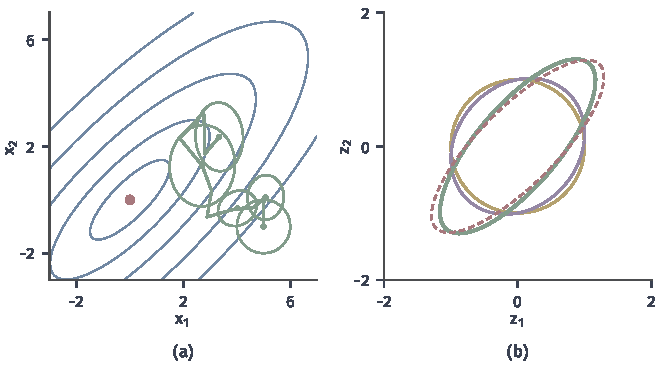
\includegraphics[width=112mm]{figures/05-optimization/05-stochastic-optimization/matplotlib/rs-cma-adapt/figure.pdf}
 \caption{CMA-ES在式~\eqref{eq:rs-rotated}上的一次运行，默认参数，$\lambda=6$，种子固定。(a)蓝线是等高线，绿线是中心的路径，绿色椭圆是第$0,2,4,7,11$代的$\sigma\bm{\Sigma}^{1/2}$单位圆像。(b)把$\bm{\Sigma}$的行列式归一化后的形状：黄线第$0$代，紫线第$6$代，绿线第$40$代，红色虚线是同样归一化的$\bm{A}^{-1}$。}
 \label{fig:rs-cma-adapt}
\end{BookInlineFigure}

在二次目标上，$\bm{\Sigma}$大致正比于$\bm{A}^{-1}$是可以理解的：作坐标变换$\bm{u}=\bm{A}^{1/2}\bm{x}$后等高线变成圆，而$\bm{\Sigma}\propto\bm{A}^{-1}$的抽样在$\bm{u}$坐标下正好是各向同性的。但这是对运行结果的描述，并不是一个无条件的等式。

一个简单的论证说明两者不可能恒等。CMA-ES只用排序，所以把$f$换成任何严格递增的函数，比如$h=\sqrt{f}$，排序完全不变，同一组随机数给出完全相同的$\bm{\Sigma}$序列。可是在$f>0$的点，
\[
 \nabla^2h=\frac{1}{2\sqrt{f}}\nabla^2f-\frac{1}{4f^{3/2}}\nabla f\nabla f^\top,
\]
它与$\nabla^2f$的形状不同。同一个$\bm{\Sigma}$不能同时是两者的逆。所以搜索协方差不是目标的Hessian，也不无条件地等于它的逆；它记录的是最近一段时间里选中位移的分布，并且依赖种群大小和有限的代数。

只用排序的好处恰恰在这里：算法的行为不随$f$的单调变换改变。这是它与第~\ref{chap:zeroth-order-optimization}章直接用函数值大小构造方向的做法的一个区别。

\subsection{步长适应}
\label{sec:rs-es-step}

协方差$\bm{\Sigma}$描述形状，而$\sigma$描述整体尺度。把两者分开的理由是：尺度需要比形状快得多的调整。这一小节的问题是：只看选中位移，怎样判断$\sigma$太大还是太小？

\paragraph{路径长度}
连续几代的位移如果彼此同向，说明本可以走得更远，$\sigma$偏小。如果彼此反向、互相抵消，说明走过了头在来回摆动，$\sigma$偏大。

图~\ref{fig:rs-cma-path-sigma}(a)(b)画的就是这两种情形：四段长度差不多的位移，同向时首尾相接的总位移很长，来回抵消时总位移很短。所以要比较的是累计路径的长度与“位移彼此无关时的路径长度”。

\begin{BookInlineFigure}
 \centering
 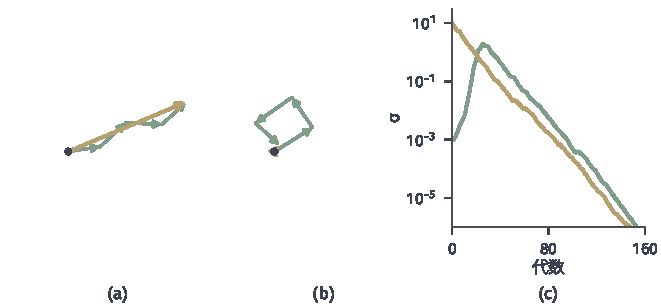
\includegraphics[width=112mm]{figures/05-optimization/05-stochastic-optimization/matplotlib/rs-cma-path-sigma/figure.pdf}
 \caption{路径长度与步长适应。(a)四段位移（绿）大致同向，累计位移（黄）长度约$4.8$。(b)四段位移互相抵消，累计位移长度约$0.2$。(c)五维球面$f=\tfrac12\lVert\bm{x}\rVert_2^2$上$\sigma$随代数的变化，只使用下面的步长路径，从$\sigma^{(0)}=10^{-3}$（绿）和$\sigma^{(0)}=10$（黄）出发，纵轴对数刻度。}
 \label{fig:rs-cma-path-sigma}
\end{BookInlineFigure}

\paragraph{标准化后累积}
为了把形状的影响除掉，累积之前先用$(\bm{\Sigma}^{(t)})^{-1/2}$把位移变成各向同性：
\begin{equation}
 \bm{p}_\sigma^{(t+1)}=(1-c_\sigma)\bm{p}_\sigma^{(t)}+\sqrt{c_\sigma(2-c_\sigma)\mu_w}\,\bigl(\bm{\Sigma}^{(t)}\bigr)^{-1/2}\bm{y}_w.
 \label{eq:rs-cma-psigma}
\end{equation}
再把路径长度与标准正态向量的期望长度比较，据此调整尺度：
\begin{equation}
 \sigma^{(t+1)}=\sigma^{(t)}\exp\Bigl(\frac{c_\sigma}{d_\sigma}\Bigl(\frac{\lVert\bm{p}_\sigma^{(t+1)}\rVert_2}{\mathbb{E}\lVert\bm{z}\rVert_2}-1\Bigr)\Bigr),\qquad\bm{z}\sim\mathcal{N}(\bm{0},\bm{I}).
 \label{eq:rs-cma-sigma}
\end{equation}
其中$d_\sigma>0$是阻尼。路径偏长时$\sigma$增大，偏短时$\sigma$减小。

系数的选取有一个清楚的理由。设选择完全随机，即排序与位移无关。这时$\bm{y}_w\sim\mathcal{N}(\bm{0},\bm{\Sigma}^{(t)}/\mu_w)$，于是$\sqrt{\mu_w}(\bm{\Sigma}^{(t)})^{-1/2}\bm{y}_w$是标准正态向量，记为$\bm{\xi}$。

若$\bm{p}_\sigma^{(t)}$也是标准正态向量，且与$\bm{\xi}$独立，那么式~\eqref{eq:rs-cma-psigma}的两项之和仍是高斯向量，协方差的系数为
\[
 (1-c_\sigma)^2+c_\sigma(2-c_\sigma)=1.
\]
所以随机选择下路径的分布不变，$\lVert\bm{p}_\sigma\rVert_2$的期望等于比较基准，$\sigma$在对数尺度上没有系统漂移。式~\eqref{eq:rs-cma-pc}的系数是同一个道理。一旦有真实选择，路径的长度偏离基准才来自评价信息。

\paragraph{例中的这一步}
接上一小节的第一代，取$c_\sigma=1/2$，$d_\sigma=1$，$\bm{\Sigma}^{(0)}=\bm{I}$，所以由式~\eqref{eq:rs-cma-psigma}，
\[
 \bm{p}_\sigma^{(1)}=1.095\,\bm{y}_w\approx\begin{bmatrix}-0.685\\-0.356\end{bmatrix},\qquad\lVert\bm{p}_\sigma^{(1)}\rVert_2\approx0.772.
\]

二维时$\bm{z}$的期望长度是$\sqrt{\pi/2}\approx1.253$。由式~\eqref{eq:rs-cma-sigma}，
\[
 \sigma^{(1)}=\exp\Bigl(\tfrac12\bigl(\tfrac{0.772}{1.253}-1\bigr)\Bigr)\approx\exp(-0.192)\approx0.825.
\]
路径比基准短，尺度缩小。第一代的路径从零开始，只积累了一代，这个判断偏保守。

图~\ref{fig:rs-cma-path-sigma}(c)是这个规则的效果。$\sigma$起初只有$10^{-3}$时，路径持续同向，$\sigma$在约$25$代内升到接近$2$；起初为$10$时，$\sigma$直接下降。之后两条线都随着接近最优点按稳定的比例减小，代价在$160$代后约为$10^{-13}$量级。

\paragraph{两条路径的职责}
两条路径形式相近，用途不同，表~\ref{tab:rs-two-paths}是对比。

\begin{BookInlineTable}
 \centering
 \caption{两条演化路径。}
 \label{tab:rs-two-paths}
 \begin{tabular}{lll}
  \toprule
  & 协方差路径$\bm{p}_c$ & 步长路径$\bm{p}_\sigma$ \\
  \midrule
  累积的量 & $\bm{y}_w$，含形状 & $\bm{\Sigma}^{-1/2}\bm{y}_w$，已标准化 \\
  用到它的什么 & 方向和符号相关 & 长度 \\
  更新谁 & $\bm{\Sigma}$（秩一项） & $\sigma$ \\
  \bottomrule
 \end{tabular}
\end{BookInlineTable}

\paragraph{更新顺序与数值处理}
一代内的次序是：抽样和评价；更新$\bm{m}$；用旧的$\bm{\Sigma}$更新$\bm{p}_\sigma$；更新$\bm{p}_c$；更新$\bm{\Sigma}$；最后更新$\sigma$。把$\bm{\Sigma}$的更新放在$\sigma$之前，是因为式~\eqref{eq:rs-cma-cov}中的$\bm{y}_{i:\lambda}$已按抽样时的$\sigma^{(t)}$标准化，这时不需要新的尺度。

实际实现还有一个小的修正：当$\lVert\bm{p}_\sigma\rVert_2$异常大，说明$\sigma$正在快速调整，这时暂停式~\eqref{eq:rs-cma-pc}右端的累积，防止形状被一次快速移动带偏。

代价方面，抽样要用$\bm{\Sigma}^{1/2}$，$\bm{p}_\sigma$要用$\bm{\Sigma}^{-1/2}$，这需要对称特征分解，稠密时一次约$O(n^3)$。通常每隔若干代才重新分解一次，把平均开销压到每次评价$O(n^2)$。

数值上要防止协方差病态：每次分解前把$\bm{\Sigma}$强制对称化，检查最小特征值是否仍为正，条件数太大时重置或停止。式~\eqref{eq:rs-cma-sigma}的指数形式保证$\sigma$恒正，无需额外处理。

\subsection{自然演化策略（补充）}
\label{sec:rs-es-nes}

前面的更新公式是逐条设计的。这一小节换一个角度：能不能把搜索分布的参数本身当作优化变量，直接写出它的梯度下降？这样得到的方法称为\term{自然演化策略}（natural evolution strategy，NES）。

\paragraph{分布参数上的目标}
设搜索分布$q_{\bm{\theta}}$由参数$\bm{\theta}$决定，把期望代价作为$\bm{\theta}$的函数：
\begin{equation}
 J(\bm{\theta})=\mathbb{E}_{\bm{x}\sim q_{\bm{\theta}}}[f(\bm{x})]=\int f(\bm{x})q_{\bm{\theta}}(\bm{x})\,\mathrm{d}\bm{x}.
 \label{eq:rs-nes-objective}
\end{equation}

$\bm{x}$可以是离散的，$f$可以不可微，只要$q_{\bm{\theta}}$对$\bm{\theta}$光滑。在可交换微分与积分的条件下，
\[
 \nabla_{\bm{\theta}}J(\bm{\theta})=\int f(\bm{x})\nabla_{\bm{\theta}}q_{\bm{\theta}}(\bm{x})\,\mathrm{d}\bm{x}.
\]

再把$\nabla q$写成$q\nabla\log q$，得到可以用样本估计的形式：
\begin{equation}
 \nabla_{\bm{\theta}}J(\bm{\theta})=\mathbb{E}_{\bm{x}\sim q_{\bm{\theta}}}\bigl[f(\bm{x})\nabla_{\bm{\theta}}\log q_{\bm{\theta}}(\bm{x})\bigr].
 \label{eq:rs-score-gradient}
\end{equation}
其中$\nabla_{\bm{\theta}}\log q_{\bm{\theta}}$称为\term{得分函数}（score function）。

\paragraph{与平滑估计的交叉}
取$q=\mathcal{N}(\bm{m},\sigma^2\bm{I})$，只把中心$\bm{m}$当参数，$\sigma$固定。写$\bm{x}=\bm{m}+\sigma\bm{z}$，得分是
\[
 \nabla_{\bm{m}}\log q=\frac{\bm{x}-\bm{m}}{\sigma^2}=\frac{\bm{z}}{\sigma}.
\]

代入式~\eqref{eq:rs-score-gradient}，有
\begin{equation}
 \nabla_{\bm{m}}J=\frac{1}{\sigma}\mathbb{E}_{\bm{z}}\bigl[f(\bm{m}+\sigma\bm{z})\bm{z}\bigr].
 \label{eq:rs-nes-gaussian}
\end{equation}
这里的$J$把$f$在$\bm{m}$周围按高斯权重做了平均，这正是第~\ref{chap:zeroth-order-optimization}章的高斯平滑目标，式~\eqref{eq:rs-nes-gaussian}正是那里的高斯方向估计。在这一实例上，分布梯度和平滑梯度是同一件事，这就是本节开头说的两种视角的重合。

一个可手算的例子：$f(x)=x^2$，$q=\mathcal{N}(m,\sigma^2)$，$m=2$，$\sigma=1$。这时精确值是$J=m^2+\sigma^2$，$\partial_mJ=2m=4$。取两个样本$z=\pm1$，读数为$f(3)=9$，$f(1)=1$，估计值为
\[
 \frac12\bigl(9\cdot1+1\cdot(-1)\bigr)=4,
\]
恰好是精确值。一般样本下估计值有方差，只有期望等于$2m$。

\paragraph{基线}
由于$\mathbb{E}[\nabla\log q]=\bm{0}$，给$f$减去一个常数$b$不改变期望，却改变方差。上例中估计量$(f(m+z)-b)z$的方差可以逐项算出。

记$a=m^2-b$，把$(m+z)^2-b$展开，估计量等于$az+2mz^2+z^3$，用$\mathbb{E}z^2=1$，$\mathbb{E}z^4=3$，$\mathbb{E}z^6=15$，奇数阶矩为零，得到
\[
 \operatorname{Var}=a^2+6a+15+8m^2.
\]

$m=2$时，$b=0$（$a=4$）的方差是$87$；$b=5$（$a=-1$）的方差是$42$；$b=7$（$a=-3$）的方差最小，是$38$。基线不改变估计的目标，只改变噪声大小。

\paragraph{自然梯度}
普通梯度依赖参数怎样写。把$\sigma$换成$\log\sigma$，梯度的方向就变了，可分布族是同一个。自然的办法是用分布之间的差别来度量参数的变化，即用\term{Fisher信息矩阵}（Fisher information matrix）
\begin{equation}
 \bm{F}(\bm{\theta})=\mathbb{E}_{\bm{x}\sim q_{\bm{\theta}}}\bigl[\nabla_{\bm{\theta}}\log q_{\bm{\theta}}(\bm{x})\nabla_{\bm{\theta}}\log q_{\bm{\theta}}(\bm{x})^\top\bigr]
 \label{eq:rs-fisher}
\end{equation}
作度量，沿\term{自然梯度}（natural gradient）下降：
\begin{equation}
 \bm{\theta}^{(t+1)}=\bm{\theta}^{(t)}-\eta\,\bm{F}(\bm{\theta}^{(t)})^{-1}\nabla_{\bm{\theta}}J(\bm{\theta}^{(t)}).
 \label{eq:rs-natural-gradient}
\end{equation}

一维高斯$\bm{\theta}=(m,\sigma)$，得分是$(z/\sigma,(z^2-1)/\sigma)$，由$\mathbb{E}z^2=1$，$\mathbb{E}(z^2-1)^2=2$，交叉项为$\mathbb{E}z(z^2-1)=0$，得
\[
 \bm{F}=\begin{bmatrix}1/\sigma^2&0\\0&2/\sigma^2\end{bmatrix}.
\]

还是目标$J=m^2+\sigma^2$，普通梯度是$(2m,2\sigma)$，自然梯度是
\[
 \bm{F}^{-1}\nabla J=(2m\sigma^2,\ \sigma^3).
\]
在$(m,\sigma)=(2,1)$，普通梯度是$(4,2)$，自然梯度是$(4,1)$。

图~\ref{fig:rs-nes-flow}比较两条连续轨迹。普通梯度沿直线同比例缩小$m$和$\sigma$。自然梯度下由$\mathrm{d}m/\mathrm{d}\sigma=2m/\sigma$得$m\propto\sigma^2$，均值比宽度收得快，分布先把中心挪到位，再缩小探索范围。

\begin{BookInlineFigure}
 \centering
 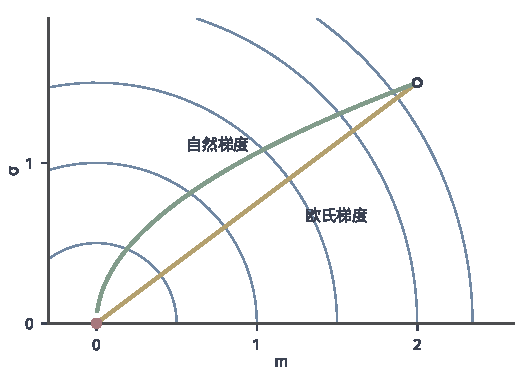
\includegraphics[width=88mm]{figures/05-optimization/05-stochastic-optimization/matplotlib/rs-nes-flow/figure.pdf}
 \caption{分布参数平面上的两条下降路径，$J(m,\sigma)=m^2+\sigma^2$，蓝线是$J$的等值线，空心圆是起点$(2,1.5)$，红点是最小点。黄线沿普通梯度，绿线沿自然梯度，后者满足$m\propto\sigma^2$。}
 \label{fig:rs-nes-flow}
\end{BookInlineFigure}

\paragraph{和CMA-ES的关系，以及要核对什么}
把$\bm{\theta}$限于中心，并把$f$换成按排序给的效用：选中的后代权重$w_i$，其余为$0$。对$\mathcal{N}(\bm{m},\sigma^2\bm{\Sigma})$，Fisher矩阵的均值块是$(\sigma^2\bm{\Sigma})^{-1}$，自然梯度下的均值更新量是
\[
 \sigma^2\bm{\Sigma}\cdot\sum_iw_i(\sigma^2\bm{\Sigma})^{-1}(\bm{x}_{i:\lambda}-\bm{m})=\sigma\sum_iw_i\bm{y}_{i:\lambda},
\]
这正是式~\eqref{eq:rs-cma-mean}。

这里有一点要小心：把$f$换成排序效用后，优化的已经不是原来的$J$，排序依赖当前样本，估计量也不再是式~\eqref{eq:rs-score-gradient}的无偏估计。基线只改变方差，排序效用改变了目标，把尺度参数写成$\sigma$还是$\log\sigma$则改变普通梯度的方向，这三件事不能混为一谈。说一个更新“是梯度下降”时，要先说清是哪个目标、哪个估计量、哪种度量。


\section{遗传算法}
\label{sec:rs-ga}

演化策略的搜索分布依赖连续变量的高斯结构，换到开关选择或排列上就用不上了。于是要问：候选是离散的编码时，怎样利用一批已评价的候选产生新的候选？\term{遗传算法}（genetic algorithm，GA）的做法是：维护一个种群，用评价选出亲代，把亲代的编码拼接和改动，得到新的候选。

“基因”“繁殖”只是沿用下来的名称。这些类比并不告诉我们一个操作在实际问题上做了什么。下面把四件事分开说明：候选的编码、亲代的选择、新候选的产生、下一代的组成。

\subsection{候选解的编码}
\label{sec:rs-ga-encoding}

遗传算法的操作都作用在编码上。这一小节的问题是：候选应当怎样写成编码，编码与原问题的解是什么关系？

\paragraph{选择问题：0--1串}
全节用一个背包问题作例子。有六件物品，第$j$件价值$v_j$、重量$w_j$，容量为$15$：
\[
 \bm{v}=(6,5,8,9,6,7),\qquad\bm{w}=(2,3,6,7,5,9).
\]

用串$\bm{b}\in\{0,1\}^6$表示选择，$b_j=1$表示选第$j$件。要最小化的是价值的相反数：
\begin{equation}
 f(\bm{b})=-\sum_{j=1}^{6}v_jb_j,\qquad\text{约束}\quad\sum_{j=1}^{6}w_jb_j\leq15.
 \label{eq:rs-knapsack}
\end{equation}
例如$\bm{b}=101100$选第$1,3,4$件，总重$15$，$f=-23$。穷举全部$2^6=64$个串可知这正是最优解，总共$30$个可行串。

\term{解码}（decoding）是从编码回到原问题的解，评价永远在解码之后进行。这里编码与解是一一对应的，解码平凡，但重量约束使得并非每个串都可行，第~\ref{sec:rs-constraints}节处理这一点。

\paragraph{顺序问题：排列}
访问顺序、任务排程的自然编码是排列，第~\ref{sec:rs-space}节的$ABDCE$就是一个例子，排列本身就是解。

把排列硬写成二进制会带来麻烦。五个元素每个用三位表示，一共$15$位，有$2^{15}=32768$种串，其中只有$5!=120$种是合法排列，约占$0.37\%$。翻一位多半得到重复元素的串，算法大部分精力花在非法候选上。

\paragraph{连续变量}
连续变量可以直接用实数向量编码，第~\ref{sec:rs-evaluation}节的比较实验就是这样做的，这时“交叉”是两个实数向量的组合，“变异”是加一个小扰动。

编码决定了什么叫“邻近”，决定了哪些操作合法，所以不存在一种通用的串表示。写清楚编码的含义、解码方式和合法操作，是这类算法要做的第一件事。

\subsection{亲代选择}
\label{sec:rs-ga-parents}

有了种群和评价，下一个问题是：谁来产生下一代的候选？选得太偏向好个体，种群很快只剩少数几种；选得太平均，又等于随机游走。用同一组数比较几种规则。设种群有$N=5$个候选，代价从好到差为
\begin{equation}
 (f_{1:5},\ldots,f_{5:5})=(-24,-20,-19,-15,-10).
 \label{eq:rs-selection-costs}
\end{equation}

\paragraph{排序选择}
把候选按代价排序，只按名次分配概率。线性排序取参数$s\in(1,2]$，第$r$名被选中的概率是
\begin{equation}
 p_r=\frac{1}{N}\Bigl(2-s+2(s-1)\frac{N-r}{N-1}\Bigr).
 \label{eq:rs-rank-selection}
\end{equation}
$s=1.5$，$N=5$时，五个名次的概率是
\[
 (0.30,\ 0.25,\ 0.20,\ 0.15,\ 0.10).
\]
由于只用名次，把代价做单调变换不影响选择。

\paragraph{锦标赛选择}
\term{锦标赛选择}（tournament selection）每次有放回地抽$k$个候选，选其中代价最小的。它不需要排序全体，也只用比较结果。第$r$名被选中，当且仅当这$k$次抽样都不比第$r$名更好（共有$N-r+1$个这样的候选可抽），并且至少有一次抽到了第$r$名。所以
\begin{equation}
 p_r=\frac{(N-r+1)^k-(N-r)^k}{N^k}.
 \label{eq:rs-tournament}
\end{equation}
这里默认没有并列。

$N=5$，$k=2$时，五个名次的概率是
\[
 (0.36,\ 0.28,\ 0.20,\ 0.12,\ 0.04).
\]

$k=3$时是
\[
 (0.488,\ 0.296,\ 0.152,\ 0.056,\ 0.008).
\]
$k$越大，好候选被选中的倾向越强。这种倾向称为\term{选择压力}（selection pressure）。以第$1$名在$N$次选择中的期望份数$Np_1$度量，$k=2$时是$1.8$份，$k=3$时是$2.44$份。

\paragraph{比例选择要先转换}
经典的比例选择把选中概率设为正比于\term{适应度}（fitness）$F$。最小化问题的代价不能直接拿来用：代价越低越好，比例却是数越大份额越大，方向就是反的。

把式~\eqref{eq:rs-selection-costs}的代价都加上$20$，问题没有变，五个数成为$(-4,0,1,5,10)$，总和是$12$，第一个比值是负数，根本不是概率。

必须先指定从代价到非负权重的转换。一种做法是以当前最差者为基准：
\begin{equation}
 F_i=f_{\max}-f_i+\delta,\qquad\delta>0.
 \label{eq:rs-fitness}
\end{equation}
取$\delta=1$，得到权重$(15,11,10,6,1)$，总和为$43$，五个概率约为
\[
 (0.349,\ 0.256,\ 0.233,\ 0.140,\ 0.023).
\]

这个转换对代价的平移不变，但概率依赖代价差的相对大小，也依赖$\delta$的取值，把$\delta$取大，选择会趋于均匀。图~\ref{fig:rs-ga-selection}把几种规则画在一起。

\begin{BookInlineFigure}
 \centering
 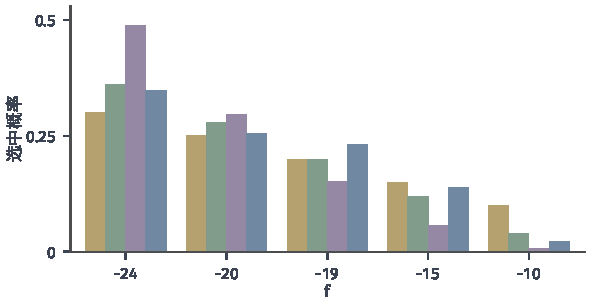
\includegraphics[width=100mm]{figures/05-optimization/05-stochastic-optimization/matplotlib/rs-ga-selection/figure.pdf}
 \caption{同一组代价~\eqref{eq:rs-selection-costs}下五个候选的选中概率，从左到右依次为线性排序（黄，$s=1.5$）、二元锦标赛（绿）、三元锦标赛（紫）、比例选择（蓝，$\delta=1$）。}
 \label{fig:rs-ga-selection}
\end{BookInlineFigure}

\subsection{交叉与变异}
\label{sec:rs-ga-operators}

选出亲代以后，怎样产生新候选？有两种操作，职责不同。\term{交叉}（crossover）把两个亲代已有的片段重新组合，只能产生两个亲代片段的拼接。\term{变异}（mutation）改动个别位置，引入亲代都没有的内容。

\paragraph{二进制串}
\textbf{单点交叉}随机选一个切点，交换切点后的尾部。用两个亲代
\[
 \bm{a}=110\,100,\qquad\bm{b}=101\,010,
\]
切点在第$3$位之后。

$\bm{b}$的前三位接$\bm{a}$的后三位，得到$101\,100$；$\bm{a}$的前三位接$\bm{b}$的后三位，得到$110\,010$。第一个后代正是最优解$101100$，$f=-23$，比两个亲代的$-20$都好。第二个后代$110010$总重$10$，$f=-17$，比两个亲代都差。交叉只是重新组合，不保证任何一个后代更好。

\textbf{逐位变异}对每一位独立以概率$p_m$翻转，常取$p_m=1/n$，平均每个串翻一位。图~\ref{fig:rs-ga-crossover}(a)中第二个后代的第$4$位翻转，变成$110110$。这个串总重$17$，超过容量，是不可行的。

\begin{BookInlineFigure}
 \centering
 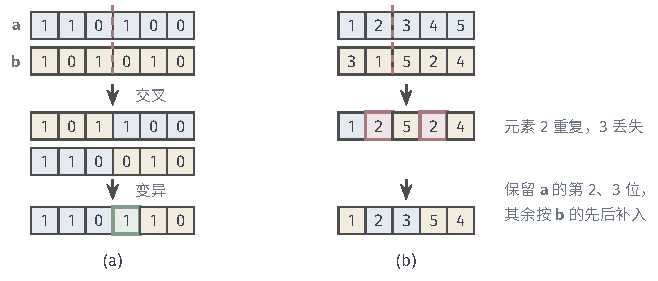
\includegraphics[width=111mm]{figures/05-optimization/05-stochastic-optimization/tikz/rs-ga-crossover/figure.pdf}
 \caption{二进制串与排列上的操作。蓝色格来自亲代$\bm{a}$，黄色格来自亲代$\bm{b}$，红色虚线是切点。(a)单点交叉后，第二个后代的第$4$位变异（绿框）。(b)在排列上直接交换尾部会产生重复元素（红框）；保留$\bm{a}$的中段再按$\bm{b}$的先后顺序补入其余元素，得到合法排列。}
 \label{fig:rs-ga-crossover}
\end{BookInlineFigure}

\paragraph{排列要用保持排列的算子}
排列上的单点交叉会出错。$\bm{a}=12345$，$\bm{b}=31524$，切点在第$2$位之后，直接拼接得到$12\,524$，元素$2$出现两次，元素$3$丢失，已经不是排列。

有两种处理办法：换用保持排列的算子，或者明确规定修复规则。\textbf{顺序交叉}属于前者：保留$\bm{a}$的第$2$、$3$位，即$23$，其余位置按$\bm{b}$中出现的先后依次填入尚未使用的元素，$\bm{b}$的顺序去掉$2,3$后是$1,5,4$，于是得到$12354$。排列上的变异也用交换两个位置或翻转一段，而不用单独改一个位置。

\paragraph{两组参数分开记录}
交叉概率$p_c$是一对亲代发生交叉的概率，不交叉时后代直接复制亲代。变异概率$p_m$是每一位翻转的概率，作用范围是一位而不是一个串。两者要分别记录。

两种操作各自都不保证改善目标。上面的例子里，同一次交叉同时给出了最好的和较差的后代，一次变异把后代变得不可行。质量的提升要靠后面的选择来累积。

\subsection{后代替换}
\label{sec:rs-ga-replacement}

亲代选择决定谁来产生新候选，后代替换决定谁进入下一代，两者是两个独立的决定。

\paragraph{三种替换}
\textbf{整代替换}用后代完全替代上一代。\term{精英保留}（elitism）在整代替换的基础上把上一代最好的若干个直接带入下一代。\textbf{逐个替换}每产生一个后代，就让它替换当前种群中最差的个体，如果它比那个个体好的话。

\needspace{6\baselineskip}
\paragraph{变量}
下面在背包问题上走完一代。要维护的量是：
\begin{itemize}
 \item 种群$\bm{b}_1,\ldots,\bm{b}_N$及其代价，$N$是种群规模；
 \item 历史最好可行解及其代价。
\end{itemize}

\paragraph{初始化}
产生初始种群并评价，这一步消耗$N$次评价。例中$N=4$，初始种群是
\[
 \begin{gathered}
 A=110100\ (\text{重}12,\ f=-20),\qquad B=101010\ (\text{重}13,\ f=-20),\\
 C=011010\ (\text{重}14,\ f=-19),\qquad D=100110\ (\text{重}14,\ f=-21).
 \end{gathered}
\]
最好记录是$D$，代价$-21$。超重的串在选择时用罚项代价$f+10\times$（超重量），第~\ref{sec:rs-constraints}节再比较其他做法。

\paragraph{每轮更新}
每一代重复以下步骤，直到预算用完。

\begin{enumerate}
 \item 用二元锦标赛选两个亲代。例中第一次比较$(B,C)$，胜者$B$；第二次比较$(A,C)$，胜者$A$。
 \item 按$p_c$决定是否交叉。例中切点在第$3$位之后，得到$101100$和$110010$。
 \item 按$p_m$逐位变异。例中第一个后代不变，第二个后代第$4$位翻转，成为$110110$。
 \item 解码并评价后代，更新历史最好可行解。例中$101100$总重$15$，$f=-23$，可行，记录更新。$110110$总重$17$，价值$26$，$f=-26$，超重$2$，罚项代价为
 \[
  -26+10\times2=-6.
 \]
 这个串的$f$虽低，却不能进入可行解的记录。
 \item 重复第1到4步，直到得到$N$个后代。例中第二对亲代的比较为$(D,A)$，胜者$D$；$(C,C)$抽到同一个候选，$C$胜出。切点在第$2$位之后，无变异，得到$101010$（$f=-20$）和$010110$（重$15$，$f=-20$）。
 \item 组成下一代。整代替换时下一代是这四个后代；精英保留一个时，$D$取代后代中最差的$110110$。
\end{enumerate}

这一代消耗$4$次评价。最终得到历史最好可行解$101100$，它是这个问题的最优解。

三种替换的结果放在表~\ref{tab:rs-ga-replacement}中。这次后代中有更好的解，三种规则的最好值都是$-23$；差别在于下一代的其余成员。如果这一代的后代都很差，整代替换会使种群的最好值变差，精英保留和逐个替换不会。

\begin{BookInlineTable}
 \centering
 \caption{同一代的三种替换结果，第三列是对应的选择用代价。}
 \label{tab:rs-ga-replacement}
 \begin{tabular}{lll}
  \toprule
  规则 & 下一代 & 代价 \\
  \midrule
  整代替换 & $101100,110110,101010,010110$ & $-23,-6,-20,-20$ \\
  精英保留 & $101100,100110,101010,010110$ & $-23,-21,-20,-20$ \\
  逐个替换 & $110100,101010,101100,100110$ & $-20,-20,-23,-21$ \\
  \bottomrule
 \end{tabular}
\end{BookInlineTable}

逐个替换那一行的过程是：$101100$替换当时最差的$C(-19)$；$110110$的$-6$比当前最差的$-20$差，不替换；后两个后代的$-20$与最差者持平，规定严格更好才替换，所以也不替换。

\paragraph{多样性的丢失}
种群有一个专门的失败方式：所有成员越来越像。把多样性度量为种群中两个不同成员平均相差的位数占总位数的比例。若某一位全种群都相同，交叉再怎么拼接，这一位也不会改变，只有变异才能恢复。

图~\ref{fig:rs-ga-diversity}在一个$40$件物品的背包问题上比较两种变异率，种群$N=30$，二元锦标赛，单点交叉，精英保留一个。没有变异时，多样性约$20$代内降到$0$，种群变成同一个串，此后每一代的后代都与亲代相同，相对最优值的间隙卡在约$15\%$。变异率$1/40$时多样性稳定在约$0.2$，$150$代后间隙约为$1.4\%$。

\begin{BookInlineFigure}
 \centering
 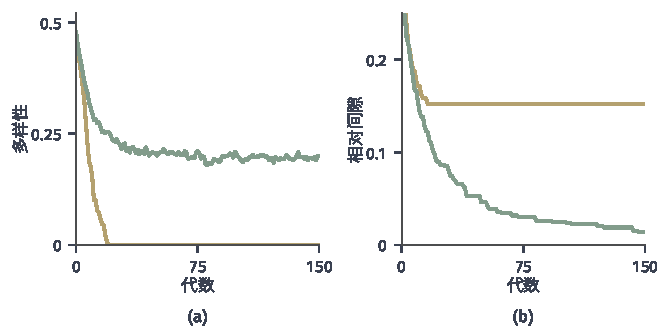
\includegraphics[width=112mm]{figures/05-optimization/05-stochastic-optimization/matplotlib/rs-ga-diversity/figure.pdf}
 \caption{$40$件物品的背包问题，$31$次运行的中位数。黄线不变异，绿线变异率$1/40$。(a)种群多样性，即两个不同成员平均相差的位数占总位数的比例。(b)历史最好可行解与最优价值的相对间隙，最优价值由动态规划算出。}
 \label{fig:rs-ga-diversity}
\end{BookInlineFigure}

保持多样性的手段有三个：变异持续注入新内容；较大的种群让位点的多样性丢失得慢；种群收敛后保留最好记录并重启。它们都消耗评价次数，要在预算内权衡。

精英保留也不能提供有限预算下的全局保证。它只保证种群的最好值不变差，这和第~\ref{sec:rs-es-selection}节的结论相同，精英甚至可能加速多样性的丢失，因为它的片段被反复选中。

\section{粒子群}
\label{sec:rs-pso}

演化策略让分布移动，遗传算法重组编码。还有一种组织方式：让每个候选都带着速度在连续空间中移动，并记住自己和同伴到过的好位置。这称为\term{粒子群优化}（particle swarm optimization，PSO）。接下来要弄清：怎样利用已发现的位置引导移动，移动的幅度由什么控制？

可以把它想成一群人在雾中找谷底，每人记得自己到过的最低处，也听得到一些同伴报告的最低处。每一步他沿惯性继续走，同时被这两个记忆的方向拉一下。这个比喻只对应更新公式的结构，不能推出任何收敛性质。

\subsection{个人与群体记忆}
\label{sec:rs-pso-memory}

粒子的移动依赖记忆。这一小节的问题是：每个粒子要记住什么，同伴之间共享什么？

\paragraph{完整状态}
设有$N$个粒子，变量是$\bm{x}\in\mathbb{R}^n$。第$i$个粒子第$t$步的状态由四个量组成：
\begin{itemize}
 \item 位置$\bm{x}_i^{(t)}$：当前候选；
 \item 速度$\bm{v}_i^{(t)}$：上一步的位移，不是目标的导数；
 \item \term{个人最好位置}（personal best）$\bm{p}_i^{(t)}$：这个粒子到过的最好位置；
 \item \term{邻域最好位置}（neighborhood best）$\bm{g}_i^{(t)}$：指定邻域内各粒子的个人最好位置中最好的一个。
\end{itemize}
本节的$\bm{g}_i$是位置，不是梯度。

初始化时在搜索区域内均匀抽位置，抽较小的初速度，评价一遍，令$\bm{p}_i^{(0)}=\bm{x}_i^{(0)}$，然后由定义得到$\bm{g}_i^{(0)}$。

个人记忆的更新规则是：
\begin{equation}
 \bm{p}_i^{(t+1)}=
 \begin{cases}
  \bm{x}_i^{(t+1)},&f(\bm{x}_i^{(t+1)})<f(\bm{p}_i^{(t)}),\\
  \bm{p}_i^{(t)},&\text{否则}.
 \end{cases}
 \label{eq:rs-pso-pbest}
\end{equation}
相同评价值时规定不更新，这样结果不依赖浮点上的偶然差别。在邻域内比较时，若有并列，按粒子编号取最小者，也要事先固定。

\paragraph{共享范围}
图~\ref{fig:rs-pso-topology}是两种共享方式。\textbf{全局共享}时所有粒子彼此相连，$\bm{g}_i$对所有$i$相同，就是全体个人记忆中最好的一个。\textbf{局部邻域}时每个粒子只与环上的相邻粒子交换信息，好位置要经过多步才能传遍全群。

\begin{BookInlineFigure}
 \centering
 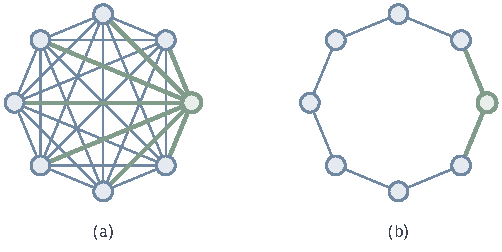
\includegraphics[width=85mm]{figures/05-optimization/05-stochastic-optimization/tikz/rs-pso-topology/figure.pdf}
 \caption{八个粒子的两种信息共享方式，绿色圆是当前关注的粒子，绿线是它能直接获知的同伴。(a)全局共享：每个粒子能看到其他所有粒子。(b)环形邻域：只与左右两个粒子交换。}
 \label{fig:rs-pso-topology}
\end{BookInlineFigure}

全局共享传播快，全群容易一起挤向同一个地方；环形邻域传播慢，不同区段可以暂时朝不同的好位置移动，保留较多的探索。

\paragraph{同步与异步}
实现上有两种顺序。\textbf{同步}更新时，一轮内所有粒子都用上一轮结束时的记忆移动，全部评价完再统一更新记忆，这便于并行评价。\textbf{异步}更新时，每评价完一个粒子，立即更新记忆，后面的粒子马上能用到新发现。两者的结果不同，记录算法时要写清楚用的是哪一种。下面用同步。

\subsection{速度与位置更新}
\label{sec:rs-pso-update}

有了状态和记忆，这一小节写出一步更新的公式，并按实际的次序算一遍。

\paragraph{主要思想}
新速度由三部分叠加：沿旧速度的惯性，朝个人记忆的拉力，朝邻域记忆的拉力。两个拉力的强度带随机性，以避免所有粒子沿同一条确定的轨迹运动：
\begin{equation}
 \begin{aligned}
 \bm{v}_i^{(t+1)}&=\bm{v}_i^{(t)}+c_1\bm{r}_{1}\odot\bigl(\bm{p}_i^{(t)}-\bm{x}_i^{(t)}\bigr)+c_2\bm{r}_{2}\odot\bigl(\bm{g}_i^{(t)}-\bm{x}_i^{(t)}\bigr),\\
 \bm{x}_i^{(t+1)}&=\bm{x}_i^{(t)}+\bm{v}_i^{(t+1)},
 \end{aligned}
 \label{eq:rs-pso-update}
\end{equation}
其中$c_1,c_2>0$是吸引系数，$\odot$表示按分量相乘，$\bm{r}_1,\bm{r}_2$的各个分量独立地均匀取自$[0,1]$，并且对每个粒子、每一轮重新抽取。

这里的差$\bm{p}_i-\bm{x}_i$和$\bm{g}_i-\bm{x}_i$只是到记忆位置的位移，不是目标的梯度。在下面的例子里$\bm{x}=(4,2)$，负梯度是$(-4,-18)$，朝邻域记忆的位移是$(-3,-1)$，两者的夹角约为$59^\circ$。粒子可以朝一个代价更高的方向飞，因为记忆里的点在那边。

\paragraph{变量}
一个粒子需要$\bm{x}$、$\bm{v}$、$\bm{p}$、$\bm{g}$，以及$f(\bm{p})$；全局还要保存历史最好记录。

\paragraph{初始化}
下面用$f(\bm{x})=\tfrac12(x_1^2+9x_2^2)$核对一步。设系数$c_1=c_2=1.5$，粒子当前状态是
\[
 \bm{x}=\begin{bmatrix}4\\2\end{bmatrix},\quad\bm{v}=\begin{bmatrix}-1\\0.5\end{bmatrix},\quad\bm{p}=\begin{bmatrix}3\\1\end{bmatrix},\quad\bm{g}=\begin{bmatrix}1\\1\end{bmatrix}.
\]
记忆处的代价是$f(\bm{p})=9$，$f(\bm{g})=5$。

\paragraph{每轮更新}
每一轮按下面的次序处理每个粒子，用完预算为止。

\begin{enumerate}
 \item 抽随机向量。例中
 \[
  \bm{r}_1=\begin{bmatrix}0.5\\0.2\end{bmatrix},\qquad\bm{r}_2=\begin{bmatrix}0.4\\0.6\end{bmatrix}.
 \]
 \item 由式~\eqref{eq:rs-pso-update}计算新速度。例中个人项和群体项分别是
 \[
  1.5\,\bm{r}_1\odot(\bm{p}-\bm{x})=\begin{bmatrix}-0.75\\-0.3\end{bmatrix},\qquad
  1.5\,\bm{r}_2\odot(\bm{g}-\bm{x})=\begin{bmatrix}-1.8\\-0.9\end{bmatrix},
 \]
 加上旧速度得到
 \[
  \bm{v}^{+}=\begin{bmatrix}-3.55\\-0.7\end{bmatrix}.
 \]
 \item 计算新位置并评价。例中
 \[
  \bm{x}^{+}=\begin{bmatrix}0.45\\1.3\end{bmatrix},\qquad f(\bm{x}^{+})=\tfrac12(0.2025+15.21)\approx7.71.
 \]
 \item 完成评价后更新记忆。例中$7.71<9$，个人记忆更新为$(0.45,1.3)$；$7.71>5$，邻域记忆$\bm{g}$不变。
\end{enumerate}

图~\ref{fig:rs-pso-vector}把这一步的三段位移画成首尾相接的箭头。这个粒子一步就把代价从$26$降到了约$7.71$，主要靠群体项。

\begin{BookInlineFigure}
 \centering
 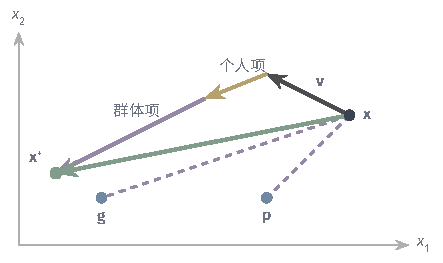
\includegraphics[width=75mm]{figures/05-optimization/05-stochastic-optimization/tikz/rs-pso-vector/figure.pdf}
 \caption{粒子的一步更新。深灰箭头是旧速度，黄箭头是个人项，紫箭头是群体项，绿箭头是合成的实际位移，虚线连向两个记忆位置。两个拉力分量的比例来自随机向量，所以合成位移不必指向任何一个记忆位置。}
 \label{fig:rs-pso-vector}
\end{BookInlineFigure}

\paragraph{速度限幅的计算}
实际常把速度各分量限制在$[-v_{\max},v_{\max}]$内。此时必须用修正后的速度计算位移。例中取$v_{\max}=2$，$\bm{v}^{+}$被截断为$(-2,-0.7)$，新位置是$(2,1.3)$，代价约为$9.61$。这比$f(\bm{p})=9$大，这一步个人记忆就不更新了。

记录下来的$\bm{v}^{+}$必须是截断后的那个，否则下一轮的惯性项与实际位移不一致。

图~\ref{fig:rs-pso-swarm}是二维Rastrigin函数上$24$个粒子的一次运行，三幅分别是第$0,8,60$轮的位置。第$8$轮粒子已聚向原点附近，第$60$轮已基本聚集，这次最好代价约为$2\times10^{-5}$。

\begin{BookInlineFigure}
 \centering
 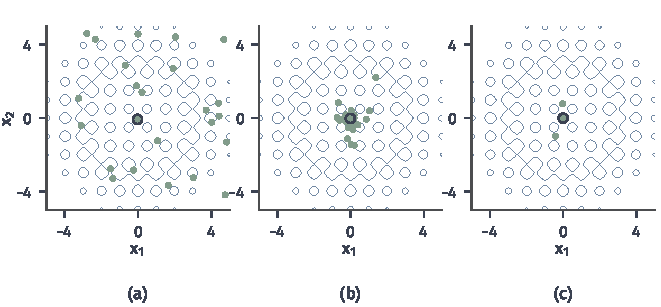
\includegraphics[width=112mm]{figures/05-optimization/05-stochastic-optimization/matplotlib/rs-pso-swarm/figure.pdf}
 \caption{二维Rastrigin函数上的粒子群，$N=24$，全局共享，带惯性权重$\omega=0.7298$，$c_1=c_2=1.496$，$v_{\max}=2$，同步更新，种子固定。(a)(b)(c)分别是第$0,8,60$轮的粒子位置（绿点），蓝线是等高线$f=30$，深色圆圈是当前的全局最好记忆，红点是全局最小点。}
 \label{fig:rs-pso-swarm}
\end{BookInlineFigure}

\subsection{移动尺度与停滞}
\label{sec:rs-pso-scale}

式~\eqref{eq:rs-pso-update}没有任何东西让速度变小。这一小节的问题是：什么控制粒子的移动尺度，粒子群停止移动时又说明了什么？

\paragraph{为什么要给速度加阻尼}
把问题简化。只看一维，记忆固定在$p=g=0$，把随机量换成常数，记$\varphi=c_1r_1+c_2r_2$。在旧速度前面乘上一个系数$\omega$（称为惯性权重），更新变成
\begin{equation}
 v^{+}=\omega v-\varphi x,\qquad x^{+}=x+v^{+}.
 \label{eq:rs-pso-deterministic}
\end{equation}
式~\eqref{eq:rs-pso-update}对应$\omega=1$。

\begin{theorem}[确定性粒子的稳定条件]
\label{thm:rs-pso-stability}
递推~\eqref{eq:rs-pso-deterministic}对任意初值都有$x^{(t)}\to0$，$v^{(t)}\to0$，当且仅当
\begin{equation}
 \lvert\omega\rvert<1,\qquad0<\varphi<2+2\omega.
 \label{eq:rs-pso-stable}
\end{equation}
\end{theorem}

\begin{proof}
把$v^{+}$代入第二式，$x^{+}=(1-\varphi)x+\omega v$，于是
\[
 \begin{bmatrix}x^{+}\\v^{+}\end{bmatrix}=\bm{M}\begin{bmatrix}x\\v\end{bmatrix},\qquad
 \bm{M}=\begin{bmatrix}1-\varphi&\omega\\-\varphi&\omega\end{bmatrix}.
\]
线性递推对任意初值收敛到零，当且仅当$\bm{M}$的两个特征值模都小于$1$。

$\bm{M}$的迹是$1-\varphi+\omega$，行列式是$\omega(1-\varphi)+\omega\varphi=\omega$，特征多项式为
\[
 \chi(z)=z^2-(1-\varphi+\omega)z+\omega.
\]

先计算两个端点的值：
\[
 \chi(1)=\varphi,\qquad\chi(-1)=2+2\omega-\varphi.
\]

两根为实数时，两根都在$(-1,1)$内，当且仅当$\chi(1)>0$，$\chi(-1)>0$，且两根之积的绝对值小于$1$，这三条合起来正是式~\eqref{eq:rs-pso-stable}。

两根为共轭复数时，$\omega>0$，模的平方等于乘积$\omega$，所以模小于$1$当且仅当$\omega<1$。此时判别式为负，给出
\[
 \lvert1-\varphi+\omega\rvert<2\sqrt{\omega}\leq1+\omega,
\]
这就是$0<\varphi<2+2\omega$，所以它自动成立。两种情形合起来，即得结论。
\end{proof}

$\omega=1$时行列式为$1$，两个特征值的模乘积为$1$，不可能都小于$1$，所以原始的式~\eqref{eq:rs-pso-update}没有衰减。图~\ref{fig:rs-pso-stability}(a)中$\omega=1$，$\varphi=1.5$的轨迹一直等幅振荡；$\omega=0.7$时振荡衰减，$45$步后已接近零。

这是把随机量换成常数后的结论，真实的$\varphi$每轮变化，乘积的稳定性与平均值的稳定性并不相同，定理只用来解释阻尼的作用。它说明了实践中必须做一件事：要么加$v_{\max}$，要么取$\omega<1$，否则粒子会越飞越散。

\begin{BookInlineFigure}
 \centering
 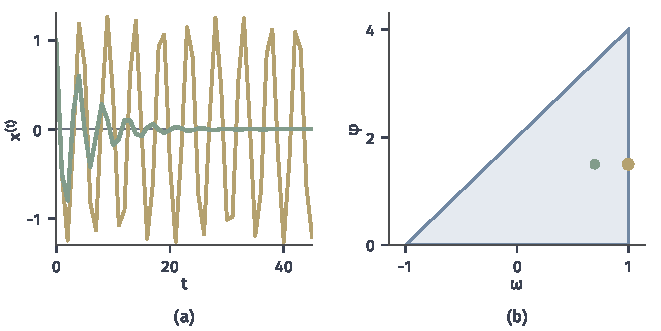
\includegraphics[width=112mm]{figures/05-optimization/05-stochastic-optimization/matplotlib/rs-pso-stability/figure.pdf}
 \caption{确定性粒子~\eqref{eq:rs-pso-deterministic}，记忆在原点，$x^{(0)}=1$，$v^{(0)}=0$。(a)$\varphi=1.5$，黄线$\omega=1$，绿线$\omega=0.7$。(b)蓝色三角形是稳定区域~\eqref{eq:rs-pso-stable}，两个点对应(a)中的两组参数，黄点位于边界上。}
 \label{fig:rs-pso-stability}
\end{BookInlineFigure}

\paragraph{三个控制量}
表~\ref{tab:rs-pso-controls}比较影响移动尺度和信息传播的三个量。它们的合适取值依赖问题和预算。

\begin{BookInlineTable}
 \centering
 \caption{粒子群的三个控制量。}
 \label{tab:rs-pso-controls}
 \begin{tabular}{lll}
  \toprule
  控制量 & 增大时 & 过度时 \\
  \midrule
  $v_{\max}$ & 允许跳得更远 & 粒子飞出搜索区域 \\
  $c_1,c_2$ & 向记忆靠拢更用力 & 振荡，越过记忆点 \\
  邻域大小 & 信息传播更快 & 全群过早聚到一处 \\
  \bottomrule
 \end{tabular}
\end{BookInlineTable}

\paragraph{越界的处理}
粒子飞出搜索区域$[\ell_j,u_j]$时，位置和速度都要处理。常用的做法是把位置截断到边界并把该分量速度置零，或者把位置反射回来并反转速度分量。

只截断位置、保留原速度是不行的：下一步粒子会继续往外冲，每一轮都贴在边界上。不管用哪一种，都要保证下一轮的$\bm{v}$与实际位移一致，这一点和速度限幅相同。第~\ref{sec:rs-constraints}节会说明，这些处理也改变了搜索的分布。

\paragraph{停滞}
考虑这样的状态：全体粒子都位于同一点$\bm{x}^\circ$，$\bm{p}_i=\bm{g}_i=\bm{x}^\circ$，$\bm{v}_i=\bm{0}$。代入式~\eqref{eq:rs-pso-update}，两个差都是零，旧速度也是零，于是不论$\bm{r}_1,\bm{r}_2$取什么值，
\[
 \bm{v}_i^{+}=\bm{0},\qquad\bm{x}_i^{+}=\bm{x}^\circ.
\]
算法从此不再移动。

这个$\bm{x}^\circ$可以是任何点。比如在$f=\tfrac12(x_1^2+9x_2^2)$上，$\bm{x}^\circ=(1,1)$的梯度是$(1,9)$，它连驻点都不是。所以粒子聚在一起、速度趋于零或者记录长期不变，都只是搜索过程的描述，不是最优性的证明。

实际运行中粒子不一定精确聚在一点，但速度变小后移动的尺度已不足以发现更好的位置，效果相同。常用的补救是重新分散一部分粒子，同时保留历史最好记录。

\section{约束处理}
\label{sec:rs-constraints}

前面几节的手算例子已经遇到了不可行的候选：背包问题里超重的串，排列交叉产生的重复元素，粒子飞出区域。这就需要回答：候选不可行时有哪些处理方式，每种方式实际上交出了什么解，又对搜索分布有什么影响？

\paragraph{先判断可行}
处理之前要能回答“这个候选在不在$\bm{C}$里”。问题~\eqref{eq:rs-problem}的$\bm{C}$通常由判定条件给出：盒约束逐分量比较上下界，排列检查元素是否恰好各出现一次，背包约束把重量加起来和容量比较。

如果判定本身需要昂贵的模拟，每次判定也要计入预算。若只有$f$的评价能告诉我们是否可行，可行性就成了评价信息的一部分。

\paragraph{直接在可行集中产生候选}
第一种方式是让操作本身不产生不可行的候选：排列上用交换和顺序交叉，盒内均匀初始化。这是最干净的做法，所有评价都用在可行候选上，不需要额外的规则。它的限制是这样的操作不总存在，一般的约束集合上没有简单的抽样办法。

\paragraph{拒绝}
第二种方式是把不可行提议直接丢弃，就当没发生，等价于把不可行候选的代价设为$+\infty$。模拟退火中，拒绝后留在原地，提议的对称性不受影响，定理~\ref{thm:rs-detailed-balance}的结论在$\bm{C}$上仍然成立，平稳分布是限制在可行集上的Gibbs分布。

代价是可行集很小时大部分提议都浪费了，并且可行集不连通时，由邻域提议连接起来的图可能分成几块，算法走不到另一块。是否花费评价次数取决于是否在判定前做函数评价，这一点要照实计入。

\paragraph{修复}
第三种方式是把不可行候选映射成一个可行候选，再评价。盒约束常用的是截断和反射；背包问题可以按价值密度$v_j/w_j$从低到高去掉物品，直到重量合格。

用遗传算法一节的不可行串$110110$演示。选中的物品是$1,2,4,5$，价值密度依次是$3$，$1.67$，$1.29$，$1.2$。去掉第$5$件后总重$12$，不超容量，得到$110100$，$f=-20$。

这时要明确记录什么。评价的是修复后的$110100$，交出去的、记入最好记录的也必须是$110100$，而不是原来的串。种群中可以存修复后的串，也可以存原串但使用修复后的评价，两种规则都可以，但要事先选定。

排列也可以修复。遗传算法一节非法的$12524$里元素$2$重复、元素$3$缺失，把第二次出现的$2$改成$3$，得到合法排列$12534$。修复规则不唯一，用哪条规则也要写明。

\paragraph{修复会改变搜索分布}
修复不是无害的。图~\ref{fig:rs-box-repair}(a)是一维的例子，当前点$x=0.1$，提议$\mathcal{N}(0.1,0.3^2)$，可行集为$[0,1]$。落到区间外的概率约$0.37$。截断把这些概率全部堆到边界$0$这一点，形成一个集中的质量；反射把区间外的部分折回区间内，密度连续；拒绝则把这部分质量留在当前点。

对称性是否保留是关键。反射后的提议密度是
\[
 \tilde q(x,y)=\sum_{k\in\mathbb{Z}}\bigl[\phi(y-x+2k)+\phi(y+x+2k)\bigr],
\]
其中$\phi$是$\mathcal{N}(0,0.3^2)$的密度。它关于$x,y$对称，所以模拟退火可以沿用式~\eqref{eq:rs-metropolis}。截断不具有这个性质。

\begin{BookInlineFigure}
 \centering
 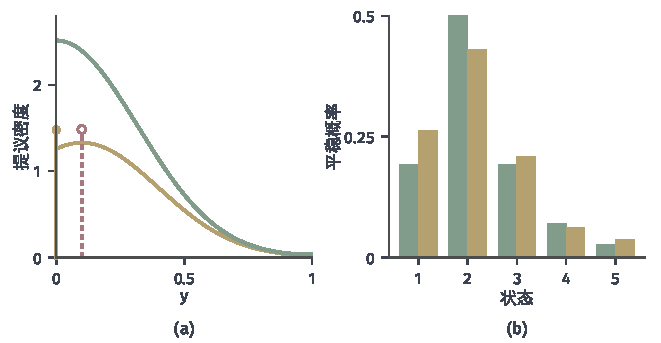
\includegraphics[width=112mm]{figures/05-optimization/05-stochastic-optimization/matplotlib/rs-box-repair/figure.pdf}
 \caption{修复对分布的影响。(a)从$x=0.1$出发的提议$\mathcal{N}(0.1,0.3^2)$在$[0,1]$上的三种处理：黄线是截断后区间内的密度，黄色竖线是截断堆积在$0$处的质量（高度为质量的$4$倍）；绿线是反射后的密度；红色虚线是拒绝时留在$x=0.1$的质量（同样放大$4$倍）。(b)五状态链的平稳分布，绿柱为Gibbs分布，黄柱是用截断提议而未修正接受概率时的实际平稳分布。}
 \label{fig:rs-box-repair}
\end{BookInlineFigure}

用离散的例子算一下。状态$\{1,\ldots,5\}$，代价$f=(1,0,1,2,3)$，$T=1$。提议从$\{-2,-1,+1,+2\}$等概率选步，超出范围就截断到端点。从$2$往左：$-1$到$1$，$-2$截断也到$1$，所以
\[
 q(2,1)=\frac12,\qquad q(1,2)=\frac14,
\]
提议不再对称。

仍用式~\eqref{eq:rs-metropolis}，实际的平稳分布约为$(0.262,0.430,0.208,0.063,0.037)$，而目标的Gibbs分布约为$(0.192,0.521,0.192,0.070,0.026)$，见图~\ref{fig:rs-box-repair}(b)。最优状态$x=2$的概率从$0.521$掉到$0.430$，边界状态的概率被抬高了。

要恢复Gibbs分布，须改用式~\eqref{eq:rs-hastings}的修正接受概率。因此模拟退火一旦带修复，就要重新核对提议与接受规则，第~\ref{sec:rs-sa-barrier}节的定理也不能直接引用。遗传算法、粒子群没有平稳分布的目标，修复的影响表现为搜索偏向边界。

\paragraph{惩罚评价}
第四种方式是把违反量折算成代价。设违反量$V(\bm{x})\geq0$，$V(\bm{x})=0$当且仅当可行，搜索时比较
\begin{equation}
 f_\rho(\bm{x})=f(\bm{x})+\rho V(\bm{x}),\qquad\rho>0.
 \label{eq:rs-penalty}
\end{equation}

系数要足够大才有用。背包问题中$V$取超重量，串$110110$的$f=-26$，$V=2$。取$\rho=1$，$f_1=-24$，低于最优可行解的$-23$，搜索会认为这个不可行的串是最好的。取$\rho=10$时是$-6$，它就排到了后面。

但$\rho$过大时，惩罚值的量级盖过$f$的差别，可行边界附近的比较失去区分度。这一取舍的系统讨论见第~\ref{chap:penalty-multiplier-methods}章。

无论$\rho$取多少，最好记录都要按式~\eqref{eq:rs-best-record}只在可行候选上更新。交出的结果若$V>0$，就要明确说明，不能和可行解的代价放在一起比较。

\paragraph{四种方式的比较}
表~\ref{tab:rs-constraints}汇总了各种方式，重点是实际返回的解。

\begin{BookInlineTable}
 \centering
 \caption{约束处理方式的比较。}
 \label{tab:rs-constraints}
 \begin{tabular}{lll}
  \toprule
  方式 & 返回的解 & 主要风险 \\
  \midrule
  可行内生成 & 原候选 & 适用的集合有限 \\
  拒绝 & 原候选 & 浪费提议，可行集分块 \\
  修复 & 修复后的候选 & 改变搜索分布 \\
  惩罚 & 原候选，须核查可行性 & 系数不当，交出不可行解 \\
  \bottomrule
 \end{tabular}
\end{BookInlineTable}

这些都是搜索算法层面的工程处理，只回答“候选不可行时算法怎么办”。约束的最优性条件、乘子和一般的约束算法由第~\ref{chap:constrained-optimality}章起的第六部分承担。


\section{含噪评价}
\label{sec:rs-noise}

到目前为止，读数都等于真实代价。如果每次评价带有噪声，如式~\eqref{eq:rs-reading}，同一个候选评价两次也会得到不同的数。噪声影响了算法的哪些环节，最好记录的含义变成了什么，额外的评价应当花在哪里？

\paragraph{噪声影响三个环节}
先明确优化的对象。本节设读数误差$\varepsilon$的均值为零，要最小化的是期望代价$f(\bm{x})=\mathbb{E}[\tilde f(\bm{x})]$；如果关心的是分位数或最坏情形，要先改定目标。这也说明，第~\ref{sec:rs-sa-barrier}节的定理和第~\ref{sec:rs-es-selection}节的单调性都是针对精确代价的，不能直接用到含噪读数上。

第一个受影响的是\textbf{接受}。设真实上坡量为$2$，$T=0.5$，无噪声时接受概率为$\mathrm{e}^{-4}\approx0.018$。若两次读数的误差各自服从$\mathcal{N}(0,1)$，接受概率的平均值变成约$0.157$，是原来的八倍多。噪声的效果相当于抬高了温度。

第二个是\textbf{排序}：种群中的名次可能和真实好坏相反，选择压力被噪声稀释。第三个是\textbf{最好记录}，这是最隐蔽的，下面专门讨论。

\paragraph{最低读数偏向有利噪声}
设有$N$个候选，真实代价都是$0$，读数相互独立，服从$\mathcal{N}(0,1)$。算法把读数最低的那个当作最好解，它的读数是$N$个标准正态变量的最小值，期望是负的。

$N=2$时可以手算。由$\min(a,b)=\tfrac12(a+b-\lvert a-b\rvert)$，两个读数$Z_1,Z_2$的最小值的期望是
\[
 \mathbb{E}\min(Z_1,Z_2)=-\tfrac12\mathbb{E}\lvert Z_1-Z_2\rvert.
\]

$Z_1-Z_2\sim\mathcal{N}(0,2)$，$\mathbb{E}\lvert Z\rvert=\sqrt{2/\pi}$，于是
\[
 \mathbb{E}\min(Z_1,Z_2)=-\tfrac12\cdot\sqrt2\cdot\sqrt{\frac2\pi}=-\frac{1}{\sqrt\pi}\approx-0.564.
\]

$N$增大，这个偏差继续变大。图~\ref{fig:rs-noise-selection}(a)显示$N=1000$时最低读数的均值约为$-3.24$，虽然所有候选的真实代价都是$0$。比较的次数越多，“最好”的读数越乐观。

\begin{BookInlineFigure}
 \centering
 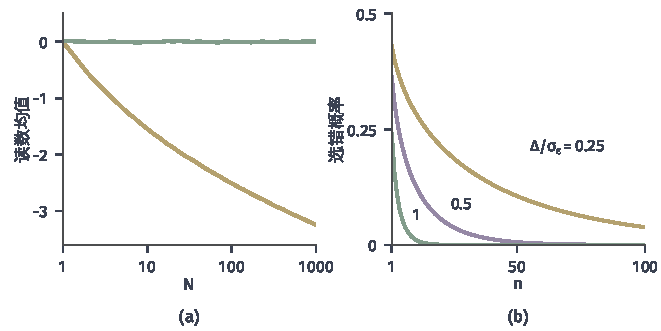
\includegraphics[width=112mm]{figures/05-optimization/05-stochastic-optimization/matplotlib/rs-noise-selection/figure.pdf}
 \caption{噪声下的选择。(a)$N$个真实代价都为$0$的候选，噪声服从$\mathcal{N}(0,1)$，黄线是最低读数的均值，绿线是对选出者重新读一次的均值，由$20000$次抽样估计。(b)两候选真实差为$\Delta$，噪声标准差为$\sigma_\varepsilon$，各读$n$次后按样本均值选错的概率，按式~\eqref{eq:rs-wrong-selection}计算。}
 \label{fig:rs-noise-selection}
\end{BookInlineFigure}

\subsection{候选比较}
\label{sec:rs-noise-compare}

两个候选的读数不同，这个差别是真的吗？这一小节讨论要读多少次才能下判断，以及读数应当分给谁。

\paragraph{重复读数}
设候选$\bm{a}$的真实代价比$\bm{b}$低$\Delta>0$。每个候选独立读$n$次，取样本均值。读数的噪声方差都是$\sigma_\varepsilon^2$时，样本均值之差的方差是$2\sigma_\varepsilon^2/n$。

样本均值之差的标准差按$1/\sqrt{n}$下降，而要分辨的真实差$\Delta$不变，所以$\Delta$越小，需要的读数越多。

\begin{theorem}[两候选比较的错误概率]
\label{thm:rs-comparison}
设两候选的读数相互独立，方差都是$\sigma_\varepsilon^2$，真实代价差为$\Delta>0$，各读$n$次后选样本均值较低者。若噪声服从高斯分布，选错的概率为
\begin{equation}
 \mathbb{P}(\text{选错})=\Phi\Bigl(-\frac{\Delta}{\sigma_\varepsilon}\sqrt{\frac{n}{2}}\Bigr),
 \label{eq:rs-wrong-selection}
\end{equation}
其中$\Phi$是标准正态分布函数。若只假定方差有限，则有
\begin{equation}
 \mathbb{P}(\text{选错})\leq\frac{2\sigma_\varepsilon^2}{n\Delta^2}.
 \label{eq:rs-wrong-chebyshev}
\end{equation}
\end{theorem}

\begin{proof}
记$\bar{a},\bar{b}$为两个样本均值，令$W=\bar{a}-\bar{b}+\Delta$，$W$的均值为$0$，方差为$2\sigma_\varepsilon^2/n$。选错即$\bar{a}\geq\bar{b}$，也就是$W\geq\Delta$。

高斯情形下$W\sim\mathcal{N}(0,2\sigma_\varepsilon^2/n)$，标准化后即得式~\eqref{eq:rs-wrong-selection}。方差有限时，由Chebyshev不等式，
\[
 \mathbb{P}(W\geq\Delta)\leq\mathbb{P}(\lvert W\rvert\geq\Delta)\leq\frac{2\sigma_\varepsilon^2}{n\Delta^2}.
\]
\end{proof}

图~\ref{fig:rs-noise-selection}(b)是式~\eqref{eq:rs-wrong-selection}。$\Delta/\sigma_\varepsilon=1$时，一次读数选错的概率约为$0.24$，$n=4$时约为$0.079$，$n=16$时约为$0.002$。$\Delta/\sigma_\varepsilon=0.5$时要$n=16$才降到$0.079$，差减半，读数要多四倍。这也就是说，$n$按$(\sigma_\varepsilon/\Delta)^2$增长。

方差未知时要用样本方差，置信水平还要计入同时比较的次数，这些统计保证的条件和推导可参考\BookChapterRef{chap:finite-sample-error-bounds}{卷八第4章“有限样本的误差上界”}。

\paragraph{把预算分给难分辨的候选}
候选的差别悬殊时，一两次读数就够分辨；差别小的，才值得多读。因此比全体平均分配读数更省的安排是：先给每个候选少量读数，计算均值和不确定性区间，淘汰区间明显落后的候选，把后续读数分给仍难分辨的那些。

这里要区分两种错误。比较误差是已见候选之间排错了名次；覆盖不足是更好的点根本没被评价过。多读几次已见的候选，只能减少前者。复核已见候选不能证明不存在更优的未见点。用于复核的读数和探索新候选竞争同一份预算，两者的分配要依问题决定。

\subsection{历史最好解的复核}
\label{sec:rs-noise-reeval}

上面看到最低读数偏向有利噪声。这一小节的问题是：对选出来的候选还能相信什么，要怎样复核？

\paragraph{选中之后重新评价}
式~\eqref{eq:rs-best-record}的记录是一次选择的结果，所以这个读数带偏。对选出的候选\textbf{用新的独立读数}重新评价，得到的就是无偏的估计。

原因是：选择只依赖旧的读数，新的噪声与选择无关。设选中的候选是$\hat{\bm{x}}$，给定$\hat{\bm{x}}$的条件下，新读数的条件期望是$f(\hat{\bm{x}})$，所以
\begin{equation}
 \mathbb{E}\bigl[\tilde f_{\mathrm{new}}(\hat{\bm{x}})\mid\hat{\bm{x}}\bigr]=f(\hat{\bm{x}}).
 \label{eq:rs-fresh-reading}
\end{equation}
图~\ref{fig:rs-noise-selection}(a)的绿线正是这一点，重新读一次的均值稳定在真实值$0$附近。

条件是新读数必须与用于选择的读数独立。把旧读数和新读数平均，偏差只是减小，并不消失。若一批复核读数又用来在多个候选中再选一次，新的选择偏差又产生了，要再留一批读数来做最终的估计。

\paragraph{新旧记录的比较}
旧记录的读数是经过多次比较选出来的最小值，新候选只有一次读数，两者并不能等量比较。$(1+1)$策略一旦遇到一次特别幸运的读数，后代的一次读数几乎都比不过它，这个亲代就长期占位，算法看起来“收敛”了，实际只是被一次噪声卡住。

常用的修正是每一代重新评价亲代，或者让记录中的候选累积多次读数后再参与比较。这些额外的评价都要计入预算，代价是每代评价数增加。

\paragraph{要记录什么}
搜索过程实际使用的选解规则要原样记录：是取最低的单次读数，还是取重复读数的最低均值，还是另留一批独立读数做最后的裁决。

报告结果时也要说清每个数字的来源。“最好值”如果是搜索过程中的最低读数，就是偏乐观的；如果来自独立的复核读数，才能作为对$f(\hat{\bm{x}})$的估计。样本复用省评价次数，但信息依赖也要一并交代。

\section{结果评价}
\label{sec:rs-evaluation}

前面每种方法都给出了手算和几幅运行图。于是要问：两种随机搜索的结果怎样比才算数，一次运行结束时能下什么结论？要把三类说法分开：有限预算内得到了什么，长期运行有什么极限性质，以及能否验证结果确实接近最优。

\subsection{停止条件}
\label{sec:rs-eval-stop}

算法要在某一刻停下来。这一小节的问题是：各种停止规则分别支持什么结论？

\paragraph{四种规则}
\textbf{评价次数上限}在用完$B$次后停止，这是最容易比较的一种。\textbf{时间上限}在规定的墙钟时间后停止，它依赖机器和实现。\textbf{目标阈值}在$f_{\mathrm{best}}\leq f_{\mathrm{target}}$时停止，要有事先给定的阈值。\textbf{停滞规则}在连续若干轮没有改善时停止。

\paragraph{停滞规则只描述已观察到的过程}
图~\ref{fig:rs-eval-budget}(c)是五维Rastrigin问题上遗传算法的一次运行。最好值从第$300$次评价前后开始，在$10.28$上停了$500$多次评价，接着又下降，最后约为$0.02$。若规则是“连续$500$次评价没有改善就停”，这次运行就会在那段平台上结束，报告$10.28$。

停滞规则说的是最近没有发现更好的点，不代表不存在更好的点。它是预算的管理手段，不是最优性的判据。分布的$\sigma$变小、粒子聚集、种群趋同也都一样。

\paragraph{有下界时报告间隙}
能证明$\ell\leq f^\star$时，可行解$\hat{\bm{x}}$的目标差不超过$f(\hat{\bm{x}})-\ell$，这是可以验证的结论，第~\ref{chap:optimization}章讨论过这种夹逼。

第~\ref{sec:rs-ga}节的背包问题就是如此：把物品按价值密度排序，允许最后一件取一部分，得到的分数背包最优值是原问题价值的上界，也就是代价的下界。那里的六件物品按价值密度排序，取第$1,2,3$件用去重量$11$，再取第$4$件的$4/7$，分数解的总价值为$19+\tfrac47\times9\approx24.14$。价值都是整数，所以$f^\star\geq-24$，最好可行解$-23$与最优值至多差$1$，这是不依赖搜索过程的结论。

大多数黑箱问题没有可靠的下界。这时老实的报告是：最好可行值是多少，用了多少次评价。不能写“达到全局最优”，因为最优值未知，而$f(\hat{\bm{x}})-f^\star$根本无从计算。

\subsection{预算与重复运行}
\label{sec:rs-eval-budget}

停下来以后要比较。这一小节的问题是：不同算法的成本怎样折算到同一单位，一次运行不够时要比较什么？

\paragraph{统一的成本单位}
不同算法的“一轮”含义不同：退火的一轮是一次评价，CMA-ES的一代是$\lambda$次，粒子群的一轮是$N$次。按轮数比较没有意义，必须换算成实际的函数调用次数。表~\ref{tab:rs-cost-accounting}列出需要计入的内容。

\begin{BookInlineTable}
 \centering
 \caption{成本的记录。第一类按评价次数统一累计，第二类另行报告。}
 \label{tab:rs-cost-accounting}
 \begin{tabular}{ll}
  \toprule
  类别 & 项目 \\
  \midrule
  函数调用 & 种群评价、退火尝试、修复后的评价 \\
  & 重复读数、最好解复核、重启 \\
  & 温度标定等试探性评价 \\
  \midrule
  内部运算 & CMA-ES的矩阵分解、排序 \\
  存储 & 种群、协方差矩阵、记忆位置 \\
  并行 & 群体通信、同步等待的时间 \\
  \bottomrule
 \end{tabular}
\end{BookInlineTable}

评价便宜时，内部运算可能反而占主导，这时只数评价次数是不够的；评价昂贵时，内部运算可以忽略。两者都要记下，分别报告。

\paragraph{结果是一个分布}
这些算法是随机的，一次运行的结果只是一个样本。比较时要固定问题、固定初始条件的抽取规则和预算，做若干次独立运行，比较结果的分布，例如中位数和四分位数。用一次最好的运行代表一个方法，或者挑选种子，都没有意义。

\paragraph{比较实验}
图~\ref{fig:rs-eval-budget}比较五种做法。问题是五维Rastrigin函数，搜索区域为$[-5.12,5.12]^5$，统一预算$B=10000$，每种方法独立运行$41$次。表~\ref{tab:rs-eval-summary}给出结束时的结果，“达标”指最好值不超过$3$。

\begin{BookInlineFigure}
 \centering
 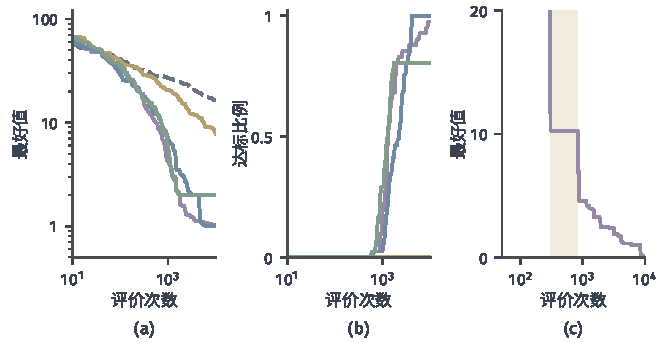
\includegraphics[width=112mm]{figures/05-optimization/05-stochastic-optimization/matplotlib/rs-eval-budget/figure.pdf}
 \caption{五维Rastrigin函数上的比较，$B=10000$，每种方法$41$次独立运行。灰色虚线为均匀随机抽样，黄线为模拟退火，紫线为实数编码遗传算法，蓝线为粒子群，绿线为CMA-ES。(a)最好值中位数随评价次数的变化。(b)最好值不超过$3$的运行所占比例。(c)遗传算法一次运行的最好值，浅黄区间是一段长约$530$次评价没有改善的平台。}
 \label{fig:rs-eval-budget}
\end{BookInlineFigure}

\begin{BookInlineTable}
 \centering
 \caption{$B=10000$时的结果（$41$次运行）。}
 \label{tab:rs-eval-summary}
 \begin{tabular}{lrrr}
  \toprule
  方法 & 中位数 & 上下四分位 & 达标比例 \\
  \midrule
  均匀随机抽样 & $16.49$ & $13.84$--$18.49$ & $0$ \\
  模拟退火 & $7.86$ & $5.69$--$10.35$ & $0$ \\
  遗传算法 & $1.03$ & $0.11$--$2.00$ & $0.98$ \\
  粒子群 & $0.99$ & $0.99$--$1.28$ & $1.00$ \\
  CMA-ES & $1.99$ & $0.99$--$2.98$ & $0.80$ \\
  \bottomrule
 \end{tabular}
\end{BookInlineTable}

这张表说明什么、不说明什么要说清楚。在这个问题、这组未专门调参的设置、这个预算下，三种基于群体或分布的方法达到了相近的量级，均匀抽样和这里的单点退火明显落后。

它不说明任何方法“更好”。退火换一组温度和提议尺度，结果可能大幅改变；CMA-ES此时已经收敛，后段的预算没有用上，加上重启可能改善；换一个问题，排序也可能颠倒。

图~\ref{fig:rs-eval-budget}(b)的曲线比一个终点数字更有信息：它回答了“要达到这个目标需要多少次评价”，三种方法都在约$10^3$次评价附近开始达标，CMA-ES的比例在约$0.8$处走平。

\paragraph{三类结论}
表~\ref{tab:rs-claims}把本章的结论按能够支持什么说法分类。写报告时，要清楚自己手里的结论属于哪一类。

\begin{BookInlineTable}
 \centering
 \caption{三类结论。}
 \label{tab:rs-claims}
 \begin{tabular}{ll}
  \toprule
  类别 & 例子与含义 \\
  \midrule
  有限预算的结果 & 中位数、达标比例：只对所测的设置成立 \\
  长期收敛结论 & 对数降温定理：是极限，并依赖模型条件 \\
  可验证的证书 & 下界与间隙：与算法如何运行无关 \\
  \bottomrule
 \end{tabular}
\end{BookInlineTable}

\section{本章小结}
\label{sec:rs-summary}

本章讨论只能评价候选时怎样组织搜索。局部改善会停在低谷，这在有限状态的双谷代价和二维多峰函数上都看得很清楚。要越过障碍，算法必须做眼前并不划算的事，四类方法的差别在于保存什么、用什么规则更新。

\textbf{模拟退火}控制单个状态的接受。对称提议下，固定温度的接受规则使Gibbs分布平稳。全局收敛定理只在有限状态、提议连通且$c\geq d^\star$的对数降温下成立，而且是概率的极限。实际的几何降温按有限预算的结果评价，温度要与代价的尺度匹配。

\textbf{演化策略}适应变异分布。保留亲代使最好值不增，整代替换允许当前值上升。CMA-ES用选中后代的加权平均移动中心，用路径和选中位移更新协方差，用标准化路径的长度调整尺度。搜索协方差不是Hessian，也不无条件等于Hessian的逆。高斯搜索分布的均值梯度与第~\ref{chap:zeroth-order-optimization}章的平滑梯度估计重合，排序效用则改变了目标。

\textbf{遗传算法}组织编码的重组与替换。编码决定什么叫邻近，排列上要用保持排列的算子，比例选择要先把代价转换为非负权重。交叉重组已有片段，变异引入新内容，没有变异时种群会完全趋同。

\textbf{粒子群}利用个人和邻域的记忆移动候选。记忆的差不是梯度，没有阻尼时确定性粒子不衰减，速度限幅后要按修正后的速度计算位移。粒子聚在一起不是最优性的证明。

各种方法要落在同一套可行性、评价信息和预算的记账上。不可行候选的处理决定了实际返回的解，修复会改变搜索分布，模拟退火须重新核对接受规则。含噪读数下最低读数偏向有利噪声，对选出的候选要用独立的新读数复核。比较方法时按实际函数调用统一预算，比较多次独立运行的结果分布。

搜索取得改善，不等于找到了全局最优。能给出下界时报告间隙，否则如实报告最好可行值和所用的预算。下一章讨论评价更昂贵的情形，用概率代理模型决定下一次评价的位置。

